\documentclass[journal, onecolumn]{IEEEtran}
\usepackage{graphicx,psfrag,epsfig,epsf,latexsym,hhline,amsmath,amssymb,amsthm}
\usepackage{url}
\interdisplaylinepenalty=2500
\oddsidemargin =0.0in
\evensidemargin=0.0in
\topmargin=-0.1in
\headsep=0.0in
\textwidth=6.5in
\textheight=9.0in

\usepackage{psfrag,epsfig,epsf,latexsym,hhline,multirow}
\usepackage{tikz,pgfplots}
\usepgflibrary{plotmarks}
\pgfplotsset{compat=newest}
\pgfplotsset{plot coordinates/math parser=false}
\usetikzlibrary{arrows,shapes,chains,matrix,positioning,scopes,patterns}
\usetikzlibrary{decorations.markings}

\newlength\figureheight 
\newlength\figurewidth

\newcommand{\mc}[1]{\mathcal{#1}}
\newcommand{\ms}[1]{\mathscr{#1}}
\newcommand{\mbb}[1]{\mathbb{#1}}
\newcommand{\mbf}[1]{\mathbf{#1}}
\newcommand{\tit}[1]{\textit{#1}}
\newcommand{\tbf}[1]{\textbf{#1}}
\newcommand{\tsc}[1]{\textsc{#1}}

\newcommand{\defeq}{\triangleq}
\newcommand{\coleq}{\mathrel{\mathop:}=}
\newcommand{\Pp}{\mathbb{P}}
\newcommand{\E}{\mathbb{E}}
\newcommand{\N}{\mathbb{N}}
\newcommand{\Z}{\mathbb{Z}}
\newcommand{\Zp}{\mathbb{Z}_{+}}
\newcommand{\R}{\mathbb{R}}
\newcommand{\Rp}{\R_{+}}
\newcommand{\g}{\mathbf{g}_}
\newcommand{\cp}{\times}
\newcommand{\Lmb}{\Lambda}
\newcommand{\lmb}{\lambda}
\newcommand{\tx}[1]{\text{#1}}

\newcommand{\Q}{\mathbb{Q}}
\newcommand{\F}{\mathbb{F}}
\newcommand{\Zw}{\mathbb{Z}[\omega]}
\newcommand{\Zi}{\mathbb{Z}[i]}
\newcommand{\C}{\mathcal{C}}

\newcommand{\abs}[1]{\lvert{#1}\rvert}
\newcommand{\card}[1]{\abs{#1}}
\newcommand{\norm}[1]{\lVert{#1}\rVert}
\newcommand{\iid}{i.\@i.\@d.\ }

\newcommand{\ceil}[1]{\lceil{#1}\rceil}
\newcommand{\floor}[1]{\lfloor{#1}\rfloor}

\DeclareMathOperator*{\argmax}{arg\,max}
\DeclareMathOperator*{\argmin}{arg\,min}

\theoremstyle{definition}\newtheorem{lemma}{Lemma}
\theoremstyle{definition}\newtheorem{proposition}[lemma]{Proposition}
\theoremstyle{definition}\newtheorem{theorem}[lemma]{Theorem}
\theoremstyle{definition}\newtheorem{corollary}[lemma]{Corollary}
\newtheorem{definition}[lemma]{Definition}
\newtheorem{Example}[lemma]{Example}
\newtheorem{Remark}[lemma]{Remark}
\newtheorem*{Discussion}{Discussion}
%\newtheorem{example}[theorem]{Example}



\newcommand{\ind}{{\rm 1\hspace*{-0.4ex}\rule{0.1ex}{1.52ex}\hspace*{0.2ex}}}
\newcommand{\dbar}[1]{\bar{\bar{#1}}}
\newcommand{\T}{\msf{T}}
\newcommand{\dotleq}{\mathrel{\dot{\leq}}}
\newcommand{\dotgeq}{\mathrel{\dot{\geq}}}
\newcommand{\dotl}{\mathrel{\dot{<}}}
\newcommand{\dotg}{\mathrel{\dot{>}}}
\newcommand{\from}{\colon}

\DeclareMathOperator{\rank}{rank}
\DeclareMathOperator{\tr}{tr}
\DeclareMathOperator{\cl}{cl}
\DeclareMathOperator{\diag}{diag}
\DeclareMathOperator{\conv}{conv}
\DeclareMathOperator{\Bernoulli}{Bernoulli}
\DeclareMathOperator{\Ei}{Ei}
\DeclareMathOperator{\OR}{OR}
\DeclareMathOperator{\Geom}{Geom}
\DeclareMathOperator{\var}{var}

\begin{document}
% Title Page
\title{Determining Minimum Energy Configurations for Constrained Membrane Problems using Two-Dimensional Message-Passing Algorithms}
\author{Avinash Vem, Krishna R. Narayanan and Arun R. Srinivasa\\
Texas A\&M University\\
College Station, TX 77843}
\maketitle


\begin{abstract}
In this work, we present a technique to find approximate minimum energy configurations of a 2-dimensional membrane using a local message-passing algorithm on the graphical structure equivalent of the membrane. This approach neither requires the energy function to be convex nor the computation of gradients. However, the disadvantage with this approach is it does not always guarantee convergence to a fixed point or a local minima solution. We are currently investigating the dependence of the convergence properties of this algorithm on the type of energy function employed.
\end{abstract}

\section{Introduction}
\label{Section:Introduction}
The objective of this work is to find minimum energy configurations of certain types of elastic membranes.  The main interest is in the case when the energy function is non-convex and when the derivative of the function with respect to the location of the particles is difficult to compute.  We propose the use of locally-effective message-passing algorithms to find minimum energy configurations. Message-passing algorithms have been shown to be very effective for solving problems in a variety of areas including coding and signal processing \cite{kschischang2001factor} and artificial intelligence \cite{pearl1988probabilistic}. Doraiswamy, Narayanan and Srinivasa used an instance of a message-passing algorithm, known as the Viterbi algorithm to find minimum energy configurations for 1-dimensional (1-D) cantilever beams \cite{doraiswamy2012finding}.

In this paper, we extend this work and consider the use of message passing algorithms for finding minimum energy configurations for the 2-dimensional elastic membranes. Unlike in its 1-D counterpart, there are no optimal minimization algorithms with a complexity that scales linearly (or, even polynomially) with the number of variables in the problem. This makes the extension from the 1-D case to the 2-D case to be non-trivial.

In this work, the membrane is modeled as a set of nodes which can take one of finitely many locations (more abstractly, can be thought of as values).  The energy function to be minimized is a function of the node (particle) locations. Our approach is to first consider a graphical model for the membrane where node locations can be treated as values taking by variable nodes and the energy arising due to the interactions between nodes are modeled by placing edges between the nodes or, equivalently through a function node. Such a graphical representation enables us to use message passing algorithm and find the configurations that minimize the energy.

It is well known that for graphs of finite sizes, when the underlying graph does not have cycles, locally-optimal iterative algorithms such as message passing algorithms are very effective and are guaranteed to converge. Pearl \cite{pearl1988probabilistic} indeed showed that the messages at convergence are guaranteed to give optimal assignment values.
For the case of graphs with cycles, for general energy functions, it cannot be guaranteed that the algorithm converges to a fixed point. Nevertheless, several empirical studies have demonstrated that excellent experimental results are obtained by running the message-algorithm on graphs with cycles and some convergence results on graphs with cycles are also available  \cite{weiss2001optimality}. Particularly in coding and signal processing, such message-passing algorithms have been very successful in 1-D problems \cite{kschischang2001factor}. Even though 2-D message passing algorithms have not been studied in as much detail as their 1-D counterparts, a few works in \cite{marrow2003iterative}, \cite{singla2002iterative} have shown that message passing algorithms can work well for two-dimensional signal processing problems also.	

Motivated by the success of the message-passing algorithm for these problems, we consider the application of these class of iterative algorithms on the approximated graphical model and show that it reaches local minima for a certain energy function.

The rest of the report is organized as follows. In section~\ref{Section:Message-Passing Framework}, we define a generic minimization problem on any undirected graph and give the message propagation rules for a generic cost function. In section \ref{Section:Application of Message-Passing rules to 2D Membrane}, we give the graphical equivalent of the energy minimization problem of a constrained membrane and present the message passing rules. Finally, in section \ref{Section:SimulationResults}, we present some simulation results.

\section{Message-Passing Framework}
\label{Section:Message-Passing Framework}
The general graphical framework considered for the minimization problem can be described as follows. Let the set of all vertices in a graph be defined as $\mathcal{V}$, the total energy function on the graph that is to be minimized as $E$ and the discrete set of values that are valid for any node as $\mathcal{S}$. $E$ is usually a function of the relative positions (or some other property of each node) of all the pairs of connected nodes in the graph. We denote the mapping that assigns to each node a value from $\mathcal{S}$ as  $\mathit{f}:\mc{V}\to \mc{S} $. For ease of notation we use the notations $f(n)$ and $f_{n}$ interchangeably. Let $\mathcal{N}$ denote the set of edges $\{(p,q)\}$, where $p,q \in \mathcal{V}$ are connected. For a given mapping, the total energy or also referred to as the objective function is given by:
\begin{equation}
 \tx{E}(f)= \sum\limits_{(p,q)\in \mc{N}} \tx{C}(f_p,f_q)
\label{Eqn:EnergyFunction}
\end{equation}
where $\tx{C}(f_p,f_q)$ is the cost associated with the edge $(p,q)\in \mathcal{N}$ for the given mapping $f$. The function $\tx{C}(f_p,f_q)$  is also referred to as the cost function. Our aim is to find a mapping that minimizes the objective function $\tx{E}$.

%\begin{equation*}
% \mathit{f}(n)=\mathnormal{f}_{n}  ~,\forall n \in \mathcal{V}, \mathnormal{f}_{n} \in \mathcal{S}.
%\end{equation*}

\subsection{Message-Passing Rules}
The message passing algorithm considered here works by passing messages between nodes in the graph in an iterative fashion. Each message is a vector of dimension $\card{\mc{S}}$. Let $m_{pq}^{t}$ be the message that node $p$ sends to a neighboring node $q$ at time (or, iteration) $t$. All messages at time $0$, $m_{pq}^{0}$ are initialized to zero vectors and new  messages at each iteration are computed as follows:
\begin{equation}
 m_{pq}^{t}(f_{q})=\min_{f_{p}} \left( \tx{C}(f_{p},f_{q})+ \sum_{s\in \mathcal{N}(p)\backslash q}m_{sp}^{t-1}(\mathit{f}_{p})  \right)
\label{Equation:MessagePassing}
\end{equation}
where neighborhood of $p$ is denoted by $\mathcal{N}(p)$ and is given by $\{s:(p,s)\in \mathcal{N} \}$ and $\mathcal{N}(p)\backslash q$ denotes the neighborhood of $p$ except $q$. The messages passed can be roughly thought of as follows: Consider the partial graph with just the nodes $\{q,p\}$ and also the nodes that are atmost $t-1$ levels away from the node $p$, then assuming the graph is cycle free, $ m_{pq}^{t}(f_{q})$ is the optimal energy over the partial graph when minimized over all the possible values of $p$ given the position of the node $q$ is fixed as $f_{q}$. Messages passed between the nodes according to \eqref{Equation:MessagePassing} are demonstrated in Fig.\ref{Fig:GenericMessagePassing}. After $M$ iterations, the energy vector is computed for each node according to,
\begin{equation}
e_{q}(f_{q})=\sum_{p\in \mc{N}(q)}m_{pq}^{M}(f_{q}).
\end{equation}

\begin{figure}[h!]
\centering
\input{./Figures/GenericMessagePassing}
\caption{Message from node $p$ to node $q$, $m_{pq}^{t}$, is a function of messages {$m_{sp}^{t-1}$} from all other neighbors to $p$}
\label{Fig:GenericMessagePassing}
\end{figure}


After a sufficient number of iterations, the mapping $f^{*}$ that minimizes $e_{q}(f_{q})$ individually at each node $q$ is considered th the output mapping i.e $f^{*}(q)=\argmin_{f_{q}}e_{q}(f_{q})$. There are several heuristics for determining when the iterations have converged. In this report, we simply iterate for a fixed number of iterations.

\section{Application of Message-Passing rules to 2D Membrane}
\label{Section:Application of Message-Passing rules to 2D Membrane}
To use the above described message passing framework on a 2-dimensional membrane for minimizing certain energy function, we need an equivalent discrete representation
of the membrane. We consider a simple configuration of a square membrane in shear. The membrane is of side $L$ units and is attached to rigid blocks
 along the top and bottom edges and is free along the sides. A relative displacement of $\delta$ units is imposed between the two blocks without changing their distance thus imposing a geometric sheer strain of $\frac{\delta}{L}$\%.

Let us consider a grid equivalent of the membrane where the membrane is represented by a grid of $N^{2}$ points. These $N^{2}$ nodes on the grid form  the set $\mathcal{V}$. In the limit of large $N$, grid behavior approaches the behavior of the membrane.

Any point on the grid can now be represented as $p_{i,j}$ where $0\leq i,j < N$. A particle on the membrane usually interacts with only its neighboring points and any energy function is a function of all such interactions between the particles. Therefore the  energy function considered here depends only on the relative location of a node with respect to its four adjacent neighbors. Hence, the neighborhood of any point is the set of four adjacent nodes given by
\begin{equation}
\mathcal{N}(p_{i,j})=\left\{p_{i,j-1},p_{i,j+1},p_{i-1,j},p_{i+1,j}  \right\}
\label{Eqn:Neighborhood}
\end{equation}

\subsection{Energy Function}
Before looking at message passing rules, we still need to define $\mathcal{S}$. As we have already discussed, any energy in the membrane stems from the interactions between neighboring particles. For the ease of computations we restrict valid locations for any node $p_{i,j}$ on the grid to a square centered around the node's base position $(x_{ij},y_{ij})$.  $\{(x_{ij},y_{ij}),0\leq i,j<N\}$ forms the  input to the algorithm and can be thought of as an initial guess for the positions of the particles. The accuracy of the solution depends on the size and resolution of $\mathcal{S}$. Then, the range of any mapping $f$ is
\begin{equation}
\mathcal{S}=\{-M\Delta,(-M+1)\Delta,...0,....M\Delta\}^{2}.
\end{equation}
To elaborate, given a mapping $\mathit{f}$, coordinates of any point $p_{i,j}$,are given by
 \begin{equation*}
\tilde{f}(p_{ij})=(x_{ij},y_{ij})+\mathit{f}\left(p_{ij}\right).
 \end{equation*}
\begin{figure}[t]
\centering
\scalebox{.85}{\input{./Figures/MessageTypes.tex}}
\caption{Four types of  incoming messages of iteration $t$.}
\label{Fig:MessageTypes}
\end{figure}


\begin{figure}[b]
\centering
\scalebox{.85}{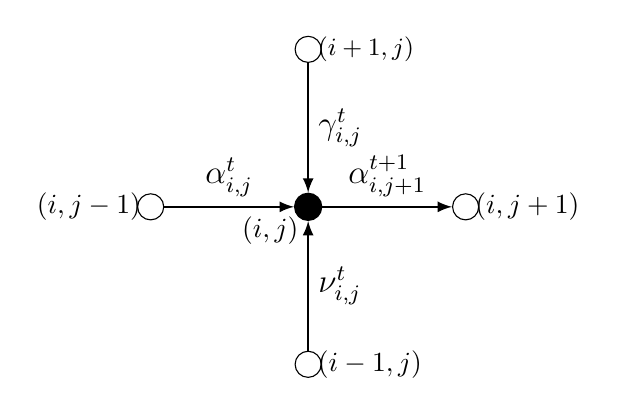
\begin{tikzpicture}[>=latex,
point/.style={circle,radius=\r,draw,thick,fill=black},
neighbor/.style={circle,radius=\r,draw}]
\def\r{0.2}
\node[point] (C) at (0,0){};
\node[neighbor] (N) at (0,2){};
\node[neighbor] (S) at (0,-2){};
\node[neighbor] (E) at (2,0) {};
\node[neighbor] (W) at (-2,0){};

\node[right] at (N) {\small{$(i+1,j)$}};
\node[right] at (S) {$(i-1,j)$};
\node[left] at (W) {$(i,j-1)$};
\node[right] at (E) {$(i,j+1)$};
\node [below left] at (C) {$(i,j)$};

\draw [thick,->] (C) to node[above]{\large{$\alpha_{i,j+1}^{t+1}$}} (E);
\draw [thick,->] (W) to node[above]{\large{$\alpha_{i,j}^{t}$}} (C);
\draw [thick,->] (N) to  node[right]{\large{$\gamma_{i,j}^{t}$}} (C);
\draw [thick,->] (S) to node[right]{\large{$\nu_{i,j}^{t}$}} (C);

\end{tikzpicture}
}
\caption{Outgoing message $\alpha_{i,j+1}^{t+1}$ as a function of the incoming messages  of iteration $t$ at node $p_{i,j}$.}
\label{Fig:OutgoingMessage}
\end{figure}

We consider the energy function,
\begin{align}
 \tx{E}(f)= &\sum_{i} \sum_{j} \tx{C}(\tilde{f}(p_{i,j}),\tilde{f}(p_{i,j-1})) + \tx{C}(\tilde{f}(p_{i,j}),\tilde{f}(p_{i,j+1})) \\ \notag
					  & +\tx{C}(\tilde{f}(p_{i,j}),\tilde{f}(p_{i-1,j})) + \tx{C}(f(p_{i,j}),\mathit{f}(p_{i+1,j}))
\end{align}
where
\begin{align}
  \tx{C}(\mbf{p}_{1},\mbf{p}_{2})&=\max \{0,\norm{\mbf{p}_{1} - \mbf{p}_{2}}^{2}-1 \} ~ \tx{ or } \notag\\
               &=\left[\norm{\mbf{p}_{1} - \mbf{p}_{2}}^{2}-1 \right]^{+}.
\label{Eqn:CostFunction1}
\end{align}
\subsection{Boundary Constraints}
The two boundaries of the grid are fixed and their co-ordinates are given by
\begin{align*}
(x_{0,j},y_{0,j})&=(j,0)  \\
(x_{N-1,j},y_{N-1,j})&=(j+\delta,N-1) ~~  0\leq j <N.
\end{align*}

The initial configuration for the nodes other than the constrained boundaries is given by
\begin{align}
x_{i,j}^{0}&=\frac{\delta}{N}i+j + \eta^{x}_{i,j} \notag\\
y_{i,j}^{0}&=j+\eta^{y}_{i,j};  i=1,2,...N-2,\forall j.\label{Eqn:InitialConfiguration}
\end{align}
where $\eta^{x}_{i,j},\eta^{y}_{i,j} \sim \mathcal{N}(0,\sigma^{2})$ are a pair of independent Gaussian random variables with zero mean and variance $ \sigma^{2}$. These noise samples help us in introducing the randomness in the initial guesses for the coordinates of the nodes. Further we model these noise samples as independent samples for any two nodes.

\subsection{Message Passing Rules}
For any point $p_{i,j}$, neighborhood defined in \eqref{Eqn:Neighborhood} consists of four points. Hence we can classify the messages in this algorithm into four types and for convenience, we use the following notation
\begin{align}
\alpha_{i,j} & := \text{Message from} \hspace{5pt} p_{i,j-1}\Rightarrow p_{i,j}~~ (\tx{West to East,})\notag \\
\beta_{i,j} & := \text{Message from} \hspace{5pt} p_{i,j+1}\Rightarrow p_{i,j}~~(\tx{East to West,})\notag \\
\gamma_{i,j} & := \text{Message from} \hspace{5pt} p_{i+1,j}\Rightarrow p_{i,j}~~(\tx{North to South,}) \notag \\
\nu_{i,j} & := \text{Message from} \hspace{5pt} p_{i-1,j}\Rightarrow p_{i,j}~(\tx{South to North}).
\label{Eqn:MessageTypesDefinition}
\end{align}

Messages defined in \eqref{Eqn:MessageTypesDefinition} are depicted in Fig. \ref{Fig:MessageTypes}.

With the above definitions, message passing rules follow directly from \eqref{Eqn:MessagePassingRules}. We give the update rules as follows:
\begin{align*}
\alpha_{i,j+1}^{t+1}(f(p_{i,j+1}))&=\min_{f(p_{i,j})}\tx{C}\big(f(p_{i,j}),f(p_{i,j+1})\big)+\alpha_{i,j}^{t}(f(p_{i,j})) +\gamma_{i,j}^{t}(f(p_{i,j})) + \nu_{i,j}^{t}(f(p_{i,j})),\\
\beta_{i,j-1}^{t+1}(f(p_{i,j-1}))&=\min_{f(p_{i,j})}\tx{C}\big(f(p_{i,j-1}),f(p_{i,j-1})\big)+\beta_{i,j}^{t}(f(p_{i,j})) +\gamma_{i,j}^{t}(f(p_{i,j})) + \nu_{i,j}^{t}(f(p_{i,j})),
\end{align*}

\begin{align}
\nu_{i+1,j}^{t+1}(f(p_{i+1,j}))&=\min_{f(p_{i,j})}\tx{C}\big(f(p_{i,j}),f(p_{i+1,j})\big)+\nu_{i,j}^{t}(f(p_{i,j})) +\alpha_{i,j}^{t}(f(p_{i,j})) + \beta_{i,j}^{t}(f(p_{i,j}))\notag\\
\gamma_{i-1,j}^{t+1}(f(p_{i-1,j}))&=\min_{f(p_{i,j})}\tx{C}\big(f(p_{i,j}),f(p_{i-1,j})\big)+\gamma_{i,j}^{t}(f(p_{i,j})) +\alpha_{i,j}^{t}(f(p_{i,j})) + \beta_{i,j}^{t}(f(p_{i,j})).\label{Eqn:MessagePassingRules}
\end{align}
Refer to Fig. \ref{Fig:OutgoingMessage} for an illustration of the message sent by node $p_{i,j}$ as a function of the messages received in previous iteration.

\section{Simulation Results}
\label{Section:SimulationResults}
\begin{figure}[h!]
\centering
% This file was created by matlab2tikz v0.4.7 running on MATLAB 7.14.
% Copyright (c) 2008--2014, Nico Schlömer <nico.schloemer@gmail.com>
% All rights reserved.
% Minimal pgfplots version: 1.3
% 
\begin{tikzpicture}[scale=0.65]
\colorlet{node color}{black}
\begin{axis}[
width=6.01828521434821in,
height=4.74667979002625in,
scale only axis,
xmin=0,
xmax=12,
xlabel={\Large{X-coordinate}},
ymin=0,
ymax=7,
ylabel={\Large{Y-coordinate}},
axis x line*=bottom,
axis y line*=left
]
\addplot[only marks,mark=*,mark options={},color=node color] plot table[row sep=crcr,]{0	0\\
0.5	0.9\\
0.9	2\\
1.5	3\\
2.1	4\\
2.7	4.9\\
3	5.8\\
3.5	7\\
1	0\\
1.6	1.1\\
2	1.7\\
2.5	2.8\\
3.1	4.3\\
3.4	4.9\\
4.1	6\\
4.5	7\\
2	0\\
2.6	1.2\\
3	1.9\\
3.8	3.2\\
3.9	3.9\\
4.4	5.2\\
4.7	6.1\\
5.5	7\\
3	0\\
3.7	1\\
4.2	1.8\\
4.5	2.8\\
5.2	3.9\\
5.5	4.9\\
6.1	5.9\\
6.5	7\\
4	0\\
4.5	1.2\\
5.1	1.9\\
5.5	3.2\\
6.6	3.9\\
6.3	5.2\\
6.6	5.9\\
7.5	7\\
5	0\\
5.3	1\\
5.8	2.2\\
6.4	2.9\\
7	3.9\\
7.5	5.4\\
8.1	6.2\\
8.5	7\\
6	0\\
6.6	0.9\\
7.2	2.1\\
7.9	2.9\\
8.2	4.1\\
8.2	5.3\\
8.5	5.7\\
9.5	7\\
7	0\\
7.7	1.2\\
7.6	2.3\\
8.5	3\\
9	4.3\\
9.9	5\\
10	5.8\\
10.5	7\\
};
\end{axis}
\end{tikzpicture}
\caption{Initial Configuration of the membrane for $N$=8, $\delta$=3.5}
\label{Fig:2D_InitialConfig}
\end{figure}

A random initial configuration for the grid is generated using \eqref{Eqn:InitialConfiguration}, and is shown in Fig. \ref{Fig:2D_InitialConfig}. Applying message passing rules as described in \eqref{Eqn:MessagePassingRules} and with 20 iterations of the algorithm, resulted in the final
configuration, shown in Fig. \ref{Fig:2D_FinalConfig}. Evolution of the value of the objective function with each iteration of message passing algorithm is shown in Fig. \ref{Fig:Energy_vs_Iterations1}.

\begin{figure}[h!]
\centering
% This file was created by matlab2tikz v0.4.7 running on MATLAB 7.14.
% Copyright (c) 2008--2014, Nico Schlömer <nico.schloemer@gmail.com>
% All rights reserved.
% Minimal pgfplots version: 1.3
% 
\
\begin{tikzpicture}[scale=0.65]
\colorlet{node color}{black}
\begin{axis}[%
width=6.01828521434821in,
height=4.74667979002625in,
scale only axis,
xmin=0,
xmax=11,
xlabel={\Large{X-coordinate}},
ymin=0,
ymax=7,
ylabel={\Large{Y-coordinate}},
axis x line*=bottom,
axis y line*=left
]
\addplot[only marks,mark=*,mark options={},color=node color] plot table[row sep=crcr,]{0	0\\
1	0\\
2	0\\
3	0\\
4	0\\
5	0\\
6	0\\
7	0\\
0.5	1\\
1.5	1\\
2.5	1\\
3.5	1\\
4.5	1\\
5.5	1\\
6.5	1\\
7.5	1\\
1	2\\
2	2\\
3	2\\
4	2\\
5	2\\
6	2\\
7	2\\
8	2\\
1.5	3\\
2.5	3\\
3.5	3\\
4.5	3\\
5.5	3\\
6.5	3\\
7.5	3\\
8.5	3\\
2	4\\
3	4\\
4	4\\
5	4\\
6	4\\
7	4\\
8	4\\
9	4\\
2.5	5\\
3.5	5\\
4.5	5\\
5.5	5\\
6.5	5\\
7.5	5\\
8.5	5\\
9.5 5\\ 
3	6\\
4	6\\
5	6\\
6	6\\
7	6\\
8	6\\
9	6\\
10	6\\
3.5	7\\
4.5	7\\
5.5	7\\
6.5 7\\
7.5	7\\
8.5	7\\
9.5	7\\
10.5	7\\
};
\end{axis}
\end{tikzpicture}%
\caption{Final Configuration after 20 iterations of message passing }
\label{Fig:2D_FinalConfig}
\end{figure}

\begin{figure}[h!]
\centering
% This file was created by matlab2tikz v0.4.7 running on MATLAB 7.14.
% Copyright (c) 2008--2014, Nico Schlömer <nico.schloemer@gmail.com>
% All rights reserved.
% Minimal pgfplots version: 1.3
% 
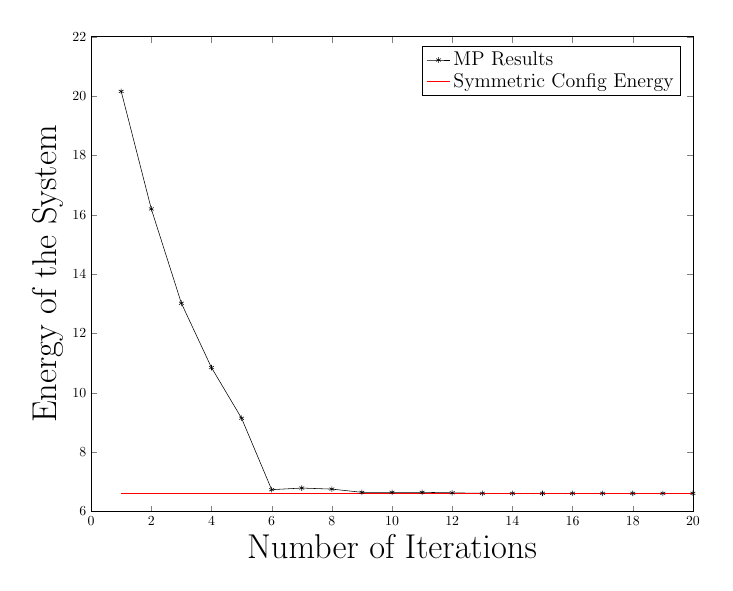
\begin{tikzpicture}[scale=0.5]

\begin{axis}[%
width=6.01828521434821in,
height=4.74667979002625in,
scale only axis,
xmin=0,
xmax=20,
xlabel={\Huge{Number of Iterations}},
ymin=6,
ymax=22,
ylabel={\Huge{Energy of the System}},
legend style={draw=black,fill=white,legend cell align=left}
]
\addplot [color=black,solid,mark=asterisk,mark options={solid}]
  table[row sep=crcr]{1	20.158516462554\\
2	16.1961617178195\\
3	13.0160697017717\\
4	10.8473134303782\\
5	9.14086714689641\\
6	6.73284434597266\\
7	6.78745526016872\\
8	6.75166418373078\\
9	6.64376023222287\\
10	6.64376023222288\\
11	6.64376023222288\\
12	6.6268318011085\\
13	6.60990336999412\\
14	6.60990336999412\\
15	6.60990336999412\\
16	6.60990336999412\\
17	6.60990336999412\\
18	6.60990336999412\\
19	6.60990336999412\\
20	6.60990336999412\\
};
\addlegendentry{\Large{MP Results}};

\addplot [color=red,solid]
  table[row sep=crcr]{1	6.60990336999411\\
2	6.60990336999411\\
3	6.60990336999411\\
4	6.60990336999411\\
5	6.60990336999411\\
6	6.60990336999411\\
7	6.60990336999411\\
8	6.60990336999411\\
9	6.60990336999411\\
10	6.60990336999411\\
11	6.60990336999411\\
12	6.60990336999411\\
13	6.60990336999411\\
14	6.60990336999411\\
15	6.60990336999411\\
16	6.60990336999411\\
17	6.60990336999411\\
18	6.60990336999411\\
19	6.60990336999411\\
20	6.60990336999411\\
};
\addlegendentry{\Large{Symmetric Config Energy}};
\end{axis}
\end{tikzpicture}
\caption{Energy versus Iterations using message passing algorithm for the 2D-Problem}
\label{Fig:Energy_vs_Iterations1}
\end{figure}

\section{An even convex Energy function}
In this section we look at the energy function $\tx{E}$ as defined previously in \eqref{Eqn:EnergyFunction} although with a different  cost function $\tx{C}$ defined as
\begin{equation}
\tx{C}(\mbf{p},\mbf{q})=\left(\abs{p_{z}-q_{z}}^{2}\right) \left(\abs{p_{z}-q_{z}}^{2}-1\right)
\label{Eqn:CostFunction2}
\end{equation}
where $p_{z}$ and $q_{z}$ are the $z$-coordinates of the respective vectors. The cost function simplifies the problem by considering just the $z$-coordinates in the cost function thus enabling us to study the shape of the membrane when a force is applied. The cost function is plotted in Fig. \ref{Fig:CostFunction2}. Observe that the above cost function has two global minima at $\abs{p_{z}-q_{z}}=\pm \frac{1}{\sqrt{2}}$.
\begin{figure}[h!]
\centering
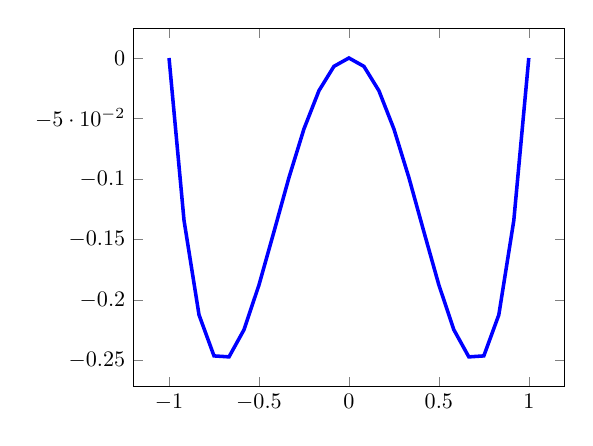
\begin{tikzpicture}[scale=0.8]
\begin{axis}
    \addplot[domain=-1:1, blue, ultra thick] { x^2*(x^2-1)};
\end{axis}
\end{tikzpicture}
\caption{Cost function vs $|p_{z}-q_{z}|$}
\label{Fig:CostFunction2}
\end{figure}

It's important to note here that sum-product message passing is an iterative algorithm that solves the problem of minimizing a function exactly on a factor graph which is equivalent to solving the optimization of a function on cycle free graphs. But the graphs we consider in this work i.e., 2D grids, are highly cyclic and hence is not guaranteed to work. For the cost function described in \eqref{Eqn:CostFunction2}, simulations showed that the message passing algorithm described above doesn't work, see Fig. \ref{Fig:Comparison_MP_Schemes}.

For this purpose we employ a message passing algorithm that uses a slightly different scheduling. First, we will describe the modified message passing algorithm used, followed by the simulation results and then the intuition behind the scheduling employed in the algorithm.

\subsection{Optimal BCJR algorithm}
Under the current setting, this problem is equivalent to finding a ML solution on a trellis code. Here's how:\\

The positions of all nodes in Rows 1 and N have been fixed. With that in mind, we will define each row as one Trellis Node making it a total of N trellis nodes and we will refer to our original nodes as normal nodes. Assuming that each normal node can has a range of values $\mathcal{S}$ as defined previously, each normal node can take any of the $|\mathcal{S}|$ values and hence each trellis node can take any of the $|\mathcal{S}|^{N}$ values from the set $\mathcal{S}^{N}=\mathcal{S} \times \mathcal{S} \cdots \times \mathcal{S}$. Any mapping $f$ assigns to each trellis node a valid state from the set $\mathcal{S}^{N}$. So hypothetically one can run a Viterbi algorithm keeping in mind the states of the inital and final trellis which are known(boundaries fixed) to us, which ideally should output the optimal solution. Note that here every set of states from the state space $\mc{S}^{N\cp N}$ is an admissible solution and hence the bit-wise optimal (Trellis node-wise optimal in this case) BCJR algorithm or the Forward-Backward algorithm is equivalent to the optimal Viterbi algorithm.
%  The problem with this is the enormously large state space($|\mathcal{S}|^{N}$ to be precise) that we have to deal with in implementing the Viterbi algorithm. Instead if we try to analyze , the task becomes simpler. 
We will introduce some notation that makes it convenient for us to describe the equivalent BCJR algorithm. The trellis-node is denoted as the vector $\mbf{p}_{i}\coleq\{p_{n,j},1\leq j \leq N\}$. Along similar lines the cost associated with a trellis-node $\mbf{p}_{i}$ is denoted as
\begin{align*}
\tx{C}\big(f(\mbf{p}_{i})\big)\coleq\sum_{j<N}\tx{C}\left(f(p_{i,j},f(p_{i,j+1})\right)
\end{align*}
 and the cost between two trellis-nodes $\mbf{p}_{i},\mbf{p}_{i+1}$ as 
 \begin{align*}
\tx{C}\big(f(\mbf{p}_{i}\leftrightarrow\mbf{p}_{i+1})\big)\coleq \sum_{j}\tx{C}\left(f(p_{i,j},p_{i+1,j})\right).
\end{align*}
With the above definitions, if one were to implement the BCJR algorithm on the equivalent trellis graph described above, the forward and backward messages can be given as follows:
\begin{align*}
\tx{E}_{\text{f}}\big(f(\mbf{p}_{n-1})\big)=\min_{f(\mbf{p}_{n-2})}\left[\tx{E}_{\text{f}}\big(f(\mbf{p}_{n-2})\big)+\tx{C}\big(f(\mbf{p}_{n-2}\leftrightarrow\mbf{p}_{n-1})\big)+\tx{C}\big(f(\mbf{p}_{n-1})\big)\right]\\
\tx{E}_{\text{b}}\big(f(\mbf{p}_{n+1})\big)=\min_{f(\mbf{p}_{n+2})}\left[\tx{E}_{\text{f}}\big(f(\mbf{p}_{n+2})\big)+\tx{C}\big(f(\mbf{p}_{n+2}\leftrightarrow\mbf{p}_{n+1})\big)+\tx{C}\big(f(\mbf{p}_{n+1})\big)\right]\\
\end{align*}
where the subscripts `$\tx{f}$' and `$\tx{b}$' in $\tx{E}_{\tx{f}}$ and $\tx{E}_{\tx{b}}$ denote the forward and backward respectively. These two quantities $\tx{E}_{\text{f}}$ and $\tx{E}_{\tx{b}}$ are the equivalents of $\alpha$ and $\beta$ messages that we deal with in BCJR or a Forward-Backward algorithm respectively. Once we have all the forward and backward messages the optimal assignment for the $n^{\tx{th}}$ trellis-node can be computed as follows:
\begin{align*}
f^*(\mbf{p}_{n})=\argmin_{f(\mbf{p}_{n})\in \mathcal{S}^{N}}\left[\tx{E}_{\text{f}}\big(f(\mbf{p}_{n-1})\big)+\tx{C}\big(f(\mbf{p}_{n-1}\leftrightarrow\mbf{p}_{n})\big)+\tx{C}\big(f(\mbf{p}_{n})\big)+\tx{C}\big(f(\mbf{p}_{n}\leftrightarrow\mbf{p}_{n+1})\big)+\tx{E}_{\text{b}}\big(f(\mbf{p}_{n+1})\big)\right].
\end{align*}
 This is how a trellis-node wise optimal algorithm for this problem would look like, but the problem here again is having to compute and store $\tx{E}_{\tx{f}}$ and $\tx{E}_{\tx{b}}$ which are vectors of size $|\mathcal{S}|^{N}$.

We employ message-passing algorithm with scheduling which closely imitates BCJR algorithm but works with vectors of size $\card{\mc{S}}$ rather than $\card{\mc{S}}^{N}$. We first describe the rules then we will explain how it is BCJR-like algorithm. 
\subsection{BCJR-like Message Passing with Scheduling}\label{Sec:MP_Scheduling}
The update rules for the messages in the vertical direction i.e the $\nu,\gamma$ messages are the same as in the normal message passing algorithm \eqref{Eqn:MessagePassingRules} whereas the messages in the horizontal direction i.e., the $\alpha, \beta$ messages follow a slightly different schedule:
\begin{align*}
\alpha_{i,j+1}^{t+1}(f(p_{i,j+1}))&=\min_{f(p_{i,j})}\left[\tx{C}\big(f(p_{i,j}),f(p_{i,j+1})\big)+\alpha_{i,j}^{t+1}(f(p_{i,j})) +\gamma_{i,j}^{t}(f(p_{i,j})) + \nu_{i,j}^{t}(f(p_{i,j})) \right]\text{ for } 1\leq j < N,\notag\\
\beta_{i,j-1}^{t+1}(f(p_{i,j-1}))&=\min_{f(p_{i,j})}\left[\tx{C}\big(f(p_{i,j-1}),f(p_{i,j-1})\big)+\beta_{i,j}^{t+1}(f(p_{i,j})) +\gamma_{i,j}^{t}(f(p_{i,j})) + \nu_{i,j}^{t}(f(p_{i,j})) \right]\text{ for } 1< j \leq N. \notag
\end{align*}

\begin{align}
\nu_{i+1,j}^{t+1}(f(p_{i+1,j}))&=\min_{f(p_{i,j})}\left[\tx{C}\big(f(p_{i,j}),f(p_{i+1,j})\big)+\nu_{i,j}^{t}(f(p_{i,j})) +\alpha_{i,j}^{t}(f(p_{i,j})) + \beta_{i,j}^{t}(f(p_{i,j}))\right]\notag\\
\gamma_{i-1,j}^{t+1}(f(p_{i-1,j}))&=\min_{f(p_{i,j})}\left[\tx{C}\big(f(p_{i,j}),f(p_{i-1,j})\big)+\gamma_{i,j}^{t}(f(p_{i,j})) +\alpha_{i,j}^{t}(f(p_{i,j})) + \beta_{i,j}^{t}(f(p_{i,j}))\right]\label{Eqn:MessagePassingRules}
\end{align}


To understand the above scheduling rules let us consider a simple grid of size $3 \times 4$ and analyze the messages received in iteration $2$ at $p_{2,3}$. %in just the horizontal direction i.e., $\alpha^{2}_{2,3}$ and $\beta^{2}_{2,3}$. This is illustrated in Fig. \ref{Fig:MP_Scheduling}. 
Recall that the initialization messages i.e., the messages sent in iteration $0$ are all zero vectors. If we analyze $\gamma_{2,3}^{2}$, it can be shown that:
\begin{align}
\gamma_{2,3}^{2}\big(f(p_{2,3})\big)&=\min_{f(p_{3,3})}\left[\alpha^{1}_{3,3}\big(f(p_{3,3})\big)+\tx{C}\big(f(p_{2,3}),f(p_{3,3})\big)+\beta^{1}_{3,3}\big(f(p_{3,3})\big)\right]\notag\\
                            &=\min_{f(p_{3,j}),j\neq 1}\left[\alpha^{1}_{3,2}\big(f(p_{3,2})\big)+\sum_{f(p_{3,j}),j> 1}\tx{C}\big( f(p_{3,j}),f(p_{3,j+1})\big)\right]\notag\\
							 &=\min_{f(\mbf{p}_{3})}\left[\tx{C}\big(f(\mbf{p}_{3})\big)+\tx{C}\big(f(p_{2,3},f(p_{3,3})\big)\right]\label{Eqn:OptimalGamma},
\end{align}
 $\gamma_{2,3}^{2}\big(f(p_{2,3})\big)$ is the value of the energy in the trellis-node $\mbf{p}_{3}$ and the edge $p_{2,3}\leftrightarrow p_{3,3}$ (all the edges shown with solid lines in top half of Fig. \ref{Fig:MP_Scheduling}) for a given $f(p_{2,3})$ and when minimized over all possible set of states for the trellis-node $\mbf{p}_{3}$. Similarly it can be shown that  $\nu_{2,3}^{2}\big(f(p_{2,3})\big)$ is the value of the energy in the trellis-node $\mbf{p}_{1}$ and the edge $p_{2,3}\leftrightarrow p_{1,3}$ (all the edges shown with solid lines in bottom half of Fig. \ref{Fig:MP_Scheduling}) for a given $f(p_{2,3})$ and when minimized over all possible set of states for the trellis-node $\mbf{p}_{1}$.
 \begin{align}
\nu_{2,3}^{2}\big(f(p_{2,3})\big) &=\min_{f(\mbf{p}_{1})}\left[\tx{C}\big(f(\mbf{p}_{1})\big)+\tx{C}\big(f(p_{2,3},f(p_{1,3})\big)\right].\label{Eqn:OptimalNu}
 \end{align}
If we consider the messages $\alpha_{2,3}^{2}$ and $\beta_{2,3}^{2}$, similar to \eqref{Eqn:OptimalGamma} and \eqref{Eqn:OptimalNu}, we can deduce that $\alpha_{2,3}^{2}\big(f(p_{2,3})\big) +\beta_{2,3}^{2}\big(f(p_{2,3})\big)$ is the energy contained in the edges shown as the dashed lines in Fig. \ref{Fig:MP_Scheduling} given $f(p_{2,3}).$
\begin{figure}[h!]
\centering
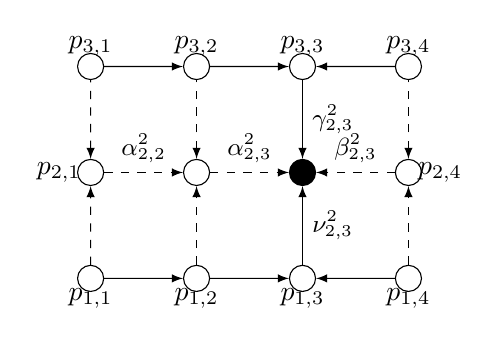
\begin{tikzpicture}[scale=0.75,>=latex,
point/.style={circle,radius=0.1,draw,fill=black},
empty/.style={circle,radius=0.1,draw,fill=none},
sha/.style={circle,radius=\r,draw,pattern=north west lines,pattern color=blue}]

\def\r{0.1}
\node[point] (23) at (0,0){};
\node[empty] (24) [right=of 23]{}
edge [dashed,->] 	node[above]	{\small{$\beta^{2}_{2,3}$}}      (23);
\node[empty] (22) [left=of 23]{}
edge [dashed,->] node[above]	{\small{$\alpha^{2}_{2,3}$}}   (23);
\node[empty] (21) [left=of 22] {}
edge [dashed,->] node[above]	{\small{$\alpha^{2}_{2,2}$}}   (22);


\node[empty] (33) [above=of 23]{}
edge [->] node[right]	{\small{$\gamma^{2}_{2,3}$}}   (23);
\node[empty] (34) [right=of 33]{}
edge [->] 	node[above]	{}(33);%\small{$\beta^{1}_{3,3}$}}      (33);
\node[empty] (32) [left=of 33]{}
edge [->] node[above]	{}(33);%\small{$\alpha^{1}_{3,3}$}}   (33);
\node[empty] (31) [left=of 32] {}
edge [->] node[above]	{}(32);%\small{$\alpha^{1}_{3,2}$}}   (32);

\node[empty] (13) [below=of 23]{}
edge [->] node[right]	{\small{$\nu^{2}_{2,3}$}}   (23);
\node[empty] (14) [right=of 13]{}
edge [->] 	node[above]	{}(13);%\small{$\beta^{1}_{1,3}$}}      (13);
\node[empty] (12) [left=of 13]{}
edge [->] node[above]	{}(13);%\small{$\alpha^{1}_{1,3}$}}   (13);
\node[empty] (11) [left=of 12] {}
edge [->] node[above]	{}(12);%\small{$\alpha^{1}_{1,2}$}}   (12);

\draw[dashed,->] (11)--(21) edge [<-,dashed] (31);
\draw[dashed,->] (12)--(22) edge [<-,dashed] (32);
\draw[dashed,->] (14)--(24) edge [<-,dashed] (34);

%\node[right] at (14){$p_{1,4}$};
\node[right] at (24){$p_{2,4}$};
\node[left] at (21) {$p_{2,1}$};

\node[above] at (31) {$p_{3,1}$};
\node[above] at (32) {$p_{3,2}$};
\node[above] at (33) {$p_{3,3}$};
\node[above] at (34){$p_{3,4}$};

\node[below] at (11) {$p_{1,1}$};
\node[below] at (12) {$p_{1,2}$};
\node[below] at (13) {$p_{1,3}$};
\node[below] at (14) {$p_{1,4}$};

\end{tikzpicture}

\caption{Messages received by $p_{2,3}$ in Iteration 2: $\gamma_{2,3}^{2}$( or $\nu_{2,3}^{2}$) is the minimum energy contained in the edges shown in solid lines in top(bottom) half when optimized over all nodes in Row 3(Row 1). See Eqns. \eqref{Eqn:OptimalGamma} and \eqref{Eqn:OptimalNu}.}
\label{Fig:MP_Scheduling}
\end{figure}
We can view $\gamma_{2,j}$ roughly as equivalent to the backward message $\tx{E}_{\tx{b}}(\mbf{p}_{3})$, $\nu_{2,j}$ roughly as equivalent to the forward message $\tx{E}_{\tx{f}}(\mbf{p}_{1})$ and $\alpha_{2,j}+\beta_{2,j}$ as the message vectors that optimize over the nodes in Row $2$ and the transitions $\mbf{p}_{2}\leftrightarrow \mbf{p}_{1}$ and $\mbf{p}_{2}\leftrightarrow \mbf{p}_{3}$ (except the edges $(p_{2,3}, p_{1,3})$ and $(p_{2,3}, p_{3,3})$. Although the optimization done by the messages $\gamma^{2}_{2,j}$ and $\alpha^{2}_{2,j}+\beta^{2}_{2,j}$ are independent they optimize over the same set of nodes $p_{3,k},k\neq j$ independently therefore leading to cycles. This leads to our belief(conjecture) that this scheduling leads to lesser number of short cycles thus improving the performance of the message passing algorithm.

\subsection{Correction Factor}
Let's assume the same grid of size $3\cp 4$ as in the example above. Consider $\nu^{3}_{3,3}$:
\begin{align*}
\nu^{4}_{3,3}\big(f(p_{3,3})\big)&=\min_{f(p_{2,3})}\left[\nu^{3}_{2,3}\big(f(p_{2,3})\big)+\alpha^{3}_{2,3}\big(f(p_{2,3})\big)+\beta^{3}_{2,3}\big(f(p_{2,3})\big)+\tx{C}\big(f(p_{2,3}),f(p_{3,3})\big)\right]\\
&=\min_{f(\mbf{p})}\left[\nu^{2}_{2,3}\big(f(p_{2,3})\big)+\sum_{j \neq 3,1\leq j \leq 4}\left[\nu^{2}_{2,j}\big(f(p_{2,j})\big)+\gamma^{2}_{2,j}\big(f(p_{2,j})\big)+\tx{C}\big(f(p_{2,j},p_{2,j+1})\big)\right]+\tx{C}\big(f(p_{2,3}),f(p_{3,3})\right]\\
\end{align*}
Notice that in the term  $\sum_{j \neq 3,1\leq j \leq M}\left[\nu^{2}_{2,j}\big(f(p_{2,j})\big)+\gamma^{2}_{2,j}\big(f(p_{2,j})\big)\right]$, the terms of the form $\nu^{2}_{2,j}$ appear for $1\leq j \leq 4$ although each term  computes approximately the same quantity $\min_{f(\mbf{p}_{1})}\left[\tx{C}\big(f(\mbf{p}_{1})\big)+\tx{C}\big(f(p_{2,j},f(p_{1,j})\big)\right]$ which leads to the addition of the term $\tx{C}\big(f(\mbf{p}_{1})\big)$ $4$ times. Thus we introduce the correction factor $\frac{1}{M}$ where the grid is of size $N \cp M$ in the computation of the messages $\gamma$ and $\nu$:
\begin{align}
\nu_{i+1,j}^{t+1}(f(p_{i+1,j}))&=\min_{f(p_{i,j})}\left[\tx{C}\big(f(p_{i,j}),f(p_{i+1,j})\big)+\frac{1}{M}\left(\nu_{i,j}^{t}(f(p_{i,j})) +\alpha_{i,j}^{t}(f(p_{i,j})) +\beta_{i,j}^{t}(f(p_{i,j}))\right)\right]\notag\\
\gamma_{i-1,j}^{t+1}(f(p_{i-1,j}))&=\min_{f(p_{i,j})}\left[\tx{C}\big(f(p_{i,j}),f(p_{i-1,j})\big)+\frac{1}{M}\left(\gamma_{i,j}^{t}(f(p_{i,j})) +\alpha_{i,j}^{t}(f(p_{i,j})) + \beta_{i,j}^{t}(f(p_{i,j}))\right)\right].
\label{Eqn:MP_Correction}
\end{align}
\begin{figure}[h]
\centering
% This file was created by matlab2tikz v0.4.7 running on MATLAB 7.14.
% Copyright (c) 2008--2014, Nico Schlömer <nico.schloemer@gmail.com>
% All rights reserved.
% Minimal pgfplots version: 1.3
% 
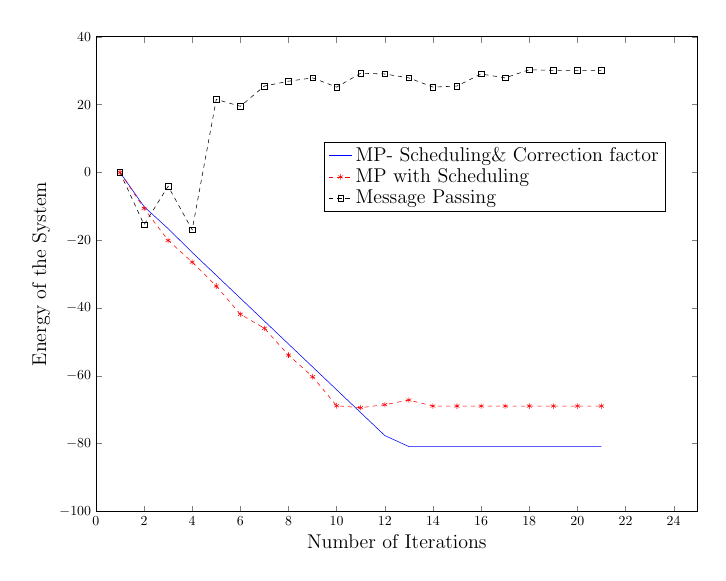
\begin{tikzpicture}[scale=0.5]

\begin{axis}[%
width=6.01828521434821in,
height=4.74667979002625in,
scale only axis,
xmin=0,
xmax=25,
xlabel={\Large{Number of Iterations}},
ymin=-100,
ymax=40,
ylabel={\Large{Energy of the System}},
legend style={at={(0.379232699914876,0.63103387411747)},anchor=south west,draw=black,fill=white,legend cell align=left}
]
\addplot [color=blue,solid]
  table[row sep=crcr]{1	0\\
2	-10.0990596517374\\
3	-16.5964932777622\\
4	-23.6087624980873\\
5	-30.3699097297178\\
6	-37.1199097297178\\
7	-43.8732855851986\\
8	-50.6232855851986\\
9	-57.3732855851986\\
10	-64.1232855851986\\
11	-70.8732855851986\\
12	-77.6232855851986\\
13	-80.8732855851986\\
14	-80.8732855851986\\
15	-80.8732855851986\\
16	-80.8732855851986\\
17	-80.8732855851986\\
18	-80.8732855851986\\
19	-80.8732855851986\\
20	-80.8732855851986\\
21	-80.8732855851986\\
};
\addlegendentry{\Large{MP- Scheduling\& Correction factor}};

\addplot [color=red,dashed,mark=asterisk,mark options={solid}]
  table[row sep=crcr]{1	0\\
2	-10.6173424187945\\
3	-20.0528427434771\\
4	-26.4699135836355\\
5	-33.5156660076328\\
6	-41.85535633809\\
7	-46.0009291488641\\
8	-53.9046651273159\\
9	-60.2570903194798\\
10	-68.8400194793213\\
11	-69.4062786463223\\
12	-68.5215306301611\\
13	-67.1621432688505\\
14	-68.9244656100818\\
15	-68.9244656100818\\
16	-68.9244656100818\\
17	-68.9244656100818\\
18	-68.9244656100818\\
19	-68.9244656100818\\
20	-68.9244656100818\\
21	-68.9244656100818\\
};
\addlegendentry{\Large{MP with Scheduling}};

\addplot [color=black,dashed,mark=square,mark options={solid}]
  table[row sep=crcr]{1	0\\
2	-15.4321252796751\\
3	-4.11191759918601\\
4	-16.944515079211\\
5	21.5232807038795\\
6	19.4843025640581\\
7	25.4578684452723\\
8	26.8812050549687\\
9	27.8691810852723\\
10	25.1434785252723\\
11	29.2304764452723\\
12	29.0124090852723\\
13	27.8691810852723\\
14	25.1434785252723\\
15	25.4578684452723\\
16	29.0124090852723\\
17	27.8691810852723\\
18	30.2683962852723\\
19	30.0811578852723\\
20	30.0811578852723\\
21	30.0811578852723\\
};
\addlegendentry{\Large{Message Passing}};

\end{axis}
\end{tikzpicture}%
\caption{Comparison of the performance of message passing versus the effects of scheduling and the correction factor included.}
\label{Fig:Comparison_MP_Schemes}
\end{figure}


\subsection{Simulation Results}
\begin{figure}[h]
\centering
\scalebox{0.75}{% This file was created by matlab2tikz v0.4.7 running on MATLAB 7.14.
% Copyright (c) 2008--2014, Nico Schlömer <nico.schloemer@gmail.com>
% All rights reserved.
% Minimal pgfplots version: 1.3
% 
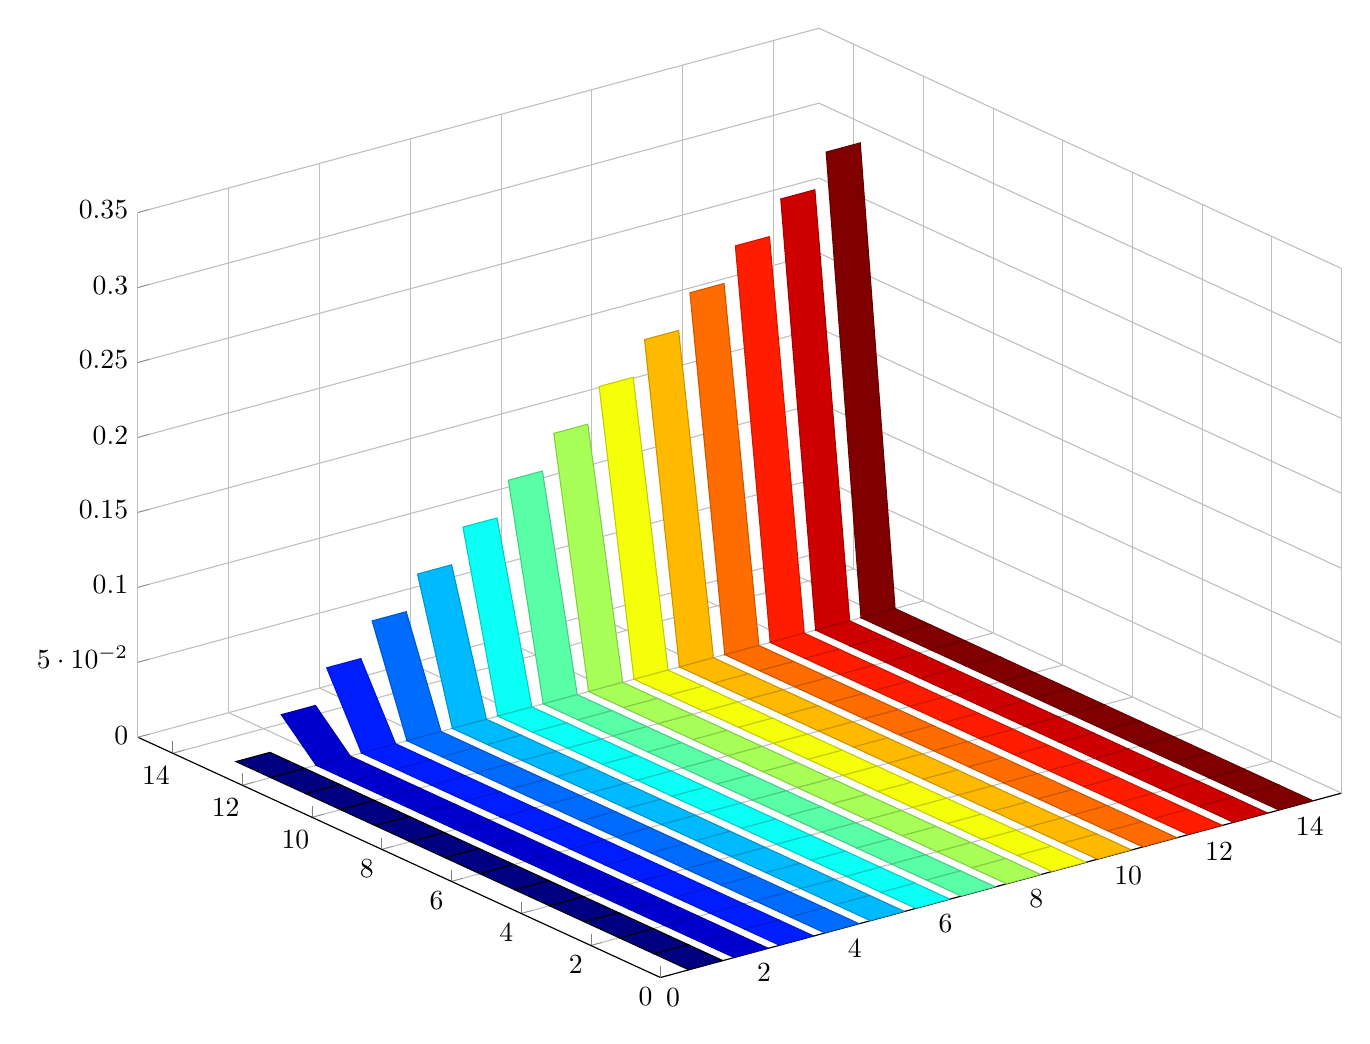
\begin{tikzpicture}

\begin{axis}[%
width=6.01828521434821in,
height=4.74667979002625in,
view={-37.5}{30},
scale only axis,
xmin=0,
xmax=15,
xmajorgrids,
ymin=0,
ymax=15,
ymajorgrids,
zmin=0,
zmax=0.35,
zmajorgrids,
axis x line*=bottom,
axis y line*=left,
axis z line*=left
]

\addplot3[%
surf,
shader=flat corner,
draw=black,
colormap/jet,
point meta=explicit,
mesh/rows=2]
table[row sep=crcr,header=false,meta index=3] {0.625	0	0	1\\
0.625	1	0	1\\
0.625	2	0	1\\
0.625	3	0	1\\
0.625	4	0	1\\
0.625	5	0	1\\
0.625	6	0	1\\
0.625	7	0	1\\
0.625	8	0	1\\
0.625	9	0	1\\
0.625	10	0	1\\
0.625	11	0	1\\
0.625	12	0	1\\
0.625	13	0	1\\
1.375	0	0	1\\
1.375	1	0	1\\
1.375	2	0	1\\
1.375	3	0	1\\
1.375	4	0	1\\
1.375	5	0	1\\
1.375	6	0	1\\
1.375	7	0	1\\
1.375	8	0	1\\
1.375	9	0	1\\
1.375	10	0	1\\
1.375	11	0	1\\
1.375	12	0	1\\
1.375	13	0	1\\
};

\addplot3[%
surf,
shader=faceted,
draw=black,
colormap/jet,
point meta=explicit,
mesh/rows=2]
table[row sep=crcr,header=false,meta index=3] {1.625	0	0	2\\
1.625	1	0	2\\
1.625	2	0	2\\
1.625	3	0	2\\
1.625	4	0	2\\
1.625	5	0	2\\
1.625	6	0	2\\
1.625	7	0	2\\
1.625	8	0	2\\
1.625	9	0	2\\
1.625	10	0	2\\
1.625	11	0	2\\
1.625	12	0	2\\
1.625	13	0.0230769230769231	2\\
2.375	0	0	2\\
2.375	1	0	2\\
2.375	2	0	2\\
2.375	3	0	2\\
2.375	4	0	2\\
2.375	5	0	2\\
2.375	6	0	2\\
2.375	7	0	2\\
2.375	8	0	2\\
2.375	9	0	2\\
2.375	10	0	2\\
2.375	11	0	2\\
2.375	12	0	2\\
2.375	13	0.0230769230769231	2\\
};

\addplot3[%
surf,
shader=faceted,
draw=black,
colormap/jet,
point meta=explicit,
mesh/rows=2]
table[row sep=crcr,header=false,meta index=3] {2.625	0	0	3\\
2.625	1	0	3\\
2.625	2	0	3\\
2.625	3	0	3\\
2.625	4	0	3\\
2.625	5	0	3\\
2.625	6	0	3\\
2.625	7	0	3\\
2.625	8	0	3\\
2.625	9	0	3\\
2.625	10	0	3\\
2.625	11	0	3\\
2.625	12	0	3\\
2.625	13	0.0461538461538461	3\\
3.375	0	0	3\\
3.375	1	0	3\\
3.375	2	0	3\\
3.375	3	0	3\\
3.375	4	0	3\\
3.375	5	0	3\\
3.375	6	0	3\\
3.375	7	0	3\\
3.375	8	0	3\\
3.375	9	0	3\\
3.375	10	0	3\\
3.375	11	0	3\\
3.375	12	0	3\\
3.375	13	0.0461538461538461	3\\
};

\addplot3[%
surf,
shader=faceted,
draw=black,
colormap/jet,
point meta=explicit,
mesh/rows=2]
table[row sep=crcr,header=false,meta index=3] {3.625	0	0	4\\
3.625	1	0	4\\
3.625	2	0	4\\
3.625	3	0	4\\
3.625	4	0	4\\
3.625	5	0	4\\
3.625	6	0	4\\
3.625	7	0	4\\
3.625	8	0	4\\
3.625	9	0	4\\
3.625	10	0	4\\
3.625	11	0	4\\
3.625	12	0	4\\
3.625	13	0.0692307692307692	4\\
4.375	0	0	4\\
4.375	1	0	4\\
4.375	2	0	4\\
4.375	3	0	4\\
4.375	4	0	4\\
4.375	5	0	4\\
4.375	6	0	4\\
4.375	7	0	4\\
4.375	8	0	4\\
4.375	9	0	4\\
4.375	10	0	4\\
4.375	11	0	4\\
4.375	12	0	4\\
4.375	13	0.0692307692307692	4\\
};

\addplot3[%
surf,
shader=faceted,
draw=black,
colormap/jet,
point meta=explicit,
mesh/rows=2]
table[row sep=crcr,header=false,meta index=3] {4.625	0	0	5\\
4.625	1	0	5\\
4.625	2	0	5\\
4.625	3	0	5\\
4.625	4	0	5\\
4.625	5	0	5\\
4.625	6	0	5\\
4.625	7	0	5\\
4.625	8	0	5\\
4.625	9	0	5\\
4.625	10	0	5\\
4.625	11	0	5\\
4.625	12	0	5\\
4.625	13	0.0923076923076923	5\\
5.375	0	0	5\\
5.375	1	0	5\\
5.375	2	0	5\\
5.375	3	0	5\\
5.375	4	0	5\\
5.375	5	0	5\\
5.375	6	0	5\\
5.375	7	0	5\\
5.375	8	0	5\\
5.375	9	0	5\\
5.375	10	0	5\\
5.375	11	0	5\\
5.375	12	0	5\\
5.375	13	0.0923076923076923	5\\
};

\addplot3[%
surf,
shader=faceted,
draw=black,
colormap/jet,
point meta=explicit,
mesh/rows=2]
table[row sep=crcr,header=false,meta index=3] {5.625	0	0	6\\
5.625	1	0	6\\
5.625	2	0	6\\
5.625	3	0	6\\
5.625	4	0	6\\
5.625	5	0	6\\
5.625	6	0	6\\
5.625	7	0	6\\
5.625	8	0	6\\
5.625	9	0	6\\
5.625	10	0	6\\
5.625	11	0	6\\
5.625	12	0	6\\
5.625	13	0.115384615384615	6\\
6.375	0	0	6\\
6.375	1	0	6\\
6.375	2	0	6\\
6.375	3	0	6\\
6.375	4	0	6\\
6.375	5	0	6\\
6.375	6	0	6\\
6.375	7	0	6\\
6.375	8	0	6\\
6.375	9	0	6\\
6.375	10	0	6\\
6.375	11	0	6\\
6.375	12	0	6\\
6.375	13	0.115384615384615	6\\
};

\addplot3[%
surf,
shader=faceted,
draw=black,
colormap/jet,
point meta=explicit,
mesh/rows=2]
table[row sep=crcr,header=false,meta index=3] {6.625	0	0	7\\
6.625	1	0	7\\
6.625	2	0	7\\
6.625	3	0	7\\
6.625	4	0	7\\
6.625	5	0	7\\
6.625	6	0	7\\
6.625	7	0	7\\
6.625	8	0	7\\
6.625	9	0	7\\
6.625	10	0	7\\
6.625	11	0	7\\
6.625	12	0	7\\
6.625	13	0.138461538461538	7\\
7.375	0	0	7\\
7.375	1	0	7\\
7.375	2	0	7\\
7.375	3	0	7\\
7.375	4	0	7\\
7.375	5	0	7\\
7.375	6	0	7\\
7.375	7	0	7\\
7.375	8	0	7\\
7.375	9	0	7\\
7.375	10	0	7\\
7.375	11	0	7\\
7.375	12	0	7\\
7.375	13	0.138461538461538	7\\
};

\addplot3[%
surf,
shader=faceted,
draw=black,
colormap/jet,
point meta=explicit,
mesh/rows=2]
table[row sep=crcr,header=false,meta index=3] {7.625	0	0	8\\
7.625	1	0	8\\
7.625	2	0	8\\
7.625	3	0	8\\
7.625	4	0	8\\
7.625	5	0	8\\
7.625	6	0	8\\
7.625	7	0	8\\
7.625	8	0	8\\
7.625	9	0	8\\
7.625	10	0	8\\
7.625	11	0	8\\
7.625	12	0	8\\
7.625	13	0.161538461538462	8\\
8.375	0	0	8\\
8.375	1	0	8\\
8.375	2	0	8\\
8.375	3	0	8\\
8.375	4	0	8\\
8.375	5	0	8\\
8.375	6	0	8\\
8.375	7	0	8\\
8.375	8	0	8\\
8.375	9	0	8\\
8.375	10	0	8\\
8.375	11	0	8\\
8.375	12	0	8\\
8.375	13	0.161538461538462	8\\
};

\addplot3[%
surf,
shader=faceted,
draw=black,
colormap/jet,
point meta=explicit,
mesh/rows=2]
table[row sep=crcr,header=false,meta index=3] {8.625	0	0	9\\
8.625	1	0	9\\
8.625	2	0	9\\
8.625	3	0	9\\
8.625	4	0	9\\
8.625	5	0	9\\
8.625	6	0	9\\
8.625	7	0	9\\
8.625	8	0	9\\
8.625	9	0	9\\
8.625	10	0	9\\
8.625	11	0	9\\
8.625	12	0	9\\
8.625	13	0.184615384615385	9\\
9.375	0	0	9\\
9.375	1	0	9\\
9.375	2	0	9\\
9.375	3	0	9\\
9.375	4	0	9\\
9.375	5	0	9\\
9.375	6	0	9\\
9.375	7	0	9\\
9.375	8	0	9\\
9.375	9	0	9\\
9.375	10	0	9\\
9.375	11	0	9\\
9.375	12	0	9\\
9.375	13	0.184615384615385	9\\
};

\addplot3[%
surf,
shader=faceted,
draw=black,
colormap/jet,
point meta=explicit,
mesh/rows=2]
table[row sep=crcr,header=false,meta index=3] {9.625	0	0	10\\
9.625	1	0	10\\
9.625	2	0	10\\
9.625	3	0	10\\
9.625	4	0	10\\
9.625	5	0	10\\
9.625	6	0	10\\
9.625	7	0	10\\
9.625	8	0	10\\
9.625	9	0	10\\
9.625	10	0	10\\
9.625	11	0	10\\
9.625	12	0	10\\
9.625	13	0.207692307692308	10\\
10.375	0	0	10\\
10.375	1	0	10\\
10.375	2	0	10\\
10.375	3	0	10\\
10.375	4	0	10\\
10.375	5	0	10\\
10.375	6	0	10\\
10.375	7	0	10\\
10.375	8	0	10\\
10.375	9	0	10\\
10.375	10	0	10\\
10.375	11	0	10\\
10.375	12	0	10\\
10.375	13	0.207692307692308	10\\
};

\addplot3[%
surf,
shader=faceted,
draw=black,
colormap/jet,
point meta=explicit,
mesh/rows=2]
table[row sep=crcr,header=false,meta index=3] {10.625	0	0	11\\
10.625	1	0	11\\
10.625	2	0	11\\
10.625	3	0	11\\
10.625	4	0	11\\
10.625	5	0	11\\
10.625	6	0	11\\
10.625	7	0	11\\
10.625	8	0	11\\
10.625	9	0	11\\
10.625	10	0	11\\
10.625	11	0	11\\
10.625	12	0	11\\
10.625	13	0.230769230769231	11\\
11.375	0	0	11\\
11.375	1	0	11\\
11.375	2	0	11\\
11.375	3	0	11\\
11.375	4	0	11\\
11.375	5	0	11\\
11.375	6	0	11\\
11.375	7	0	11\\
11.375	8	0	11\\
11.375	9	0	11\\
11.375	10	0	11\\
11.375	11	0	11\\
11.375	12	0	11\\
11.375	13	0.230769230769231	11\\
};

\addplot3[%
surf,
shader=faceted,
draw=black,
colormap/jet,
point meta=explicit,
mesh/rows=2]
table[row sep=crcr,header=false,meta index=3] {11.625	0	0	12\\
11.625	1	0	12\\
11.625	2	0	12\\
11.625	3	0	12\\
11.625	4	0	12\\
11.625	5	0	12\\
11.625	6	0	12\\
11.625	7	0	12\\
11.625	8	0	12\\
11.625	9	0	12\\
11.625	10	0	12\\
11.625	11	0	12\\
11.625	12	0	12\\
11.625	13	0.253846153846154	12\\
12.375	0	0	12\\
12.375	1	0	12\\
12.375	2	0	12\\
12.375	3	0	12\\
12.375	4	0	12\\
12.375	5	0	12\\
12.375	6	0	12\\
12.375	7	0	12\\
12.375	8	0	12\\
12.375	9	0	12\\
12.375	10	0	12\\
12.375	11	0	12\\
12.375	12	0	12\\
12.375	13	0.253846153846154	12\\
};

\addplot3[%
surf,
shader=faceted,
draw=black,
colormap/jet,
point meta=explicit,
mesh/rows=2]
table[row sep=crcr,header=false,meta index=3] {12.625	0	0	13\\
12.625	1	0	13\\
12.625	2	0	13\\
12.625	3	0	13\\
12.625	4	0	13\\
12.625	5	0	13\\
12.625	6	0	13\\
12.625	7	0	13\\
12.625	8	0	13\\
12.625	9	0	13\\
12.625	10	0	13\\
12.625	11	0	13\\
12.625	12	0	13\\
12.625	13	0.276923076923077	13\\
13.375	0	0	13\\
13.375	1	0	13\\
13.375	2	0	13\\
13.375	3	0	13\\
13.375	4	0	13\\
13.375	5	0	13\\
13.375	6	0	13\\
13.375	7	0	13\\
13.375	8	0	13\\
13.375	9	0	13\\
13.375	10	0	13\\
13.375	11	0	13\\
13.375	12	0	13\\
13.375	13	0.276923076923077	13\\
};

\addplot3[%
surf,
shader=faceted,
draw=black,
colormap/jet,
point meta=explicit,
mesh/rows=2]
table[row sep=crcr,header=false,meta index=3] {13.625	0	0	14\\
13.625	1	0	14\\
13.625	2	0	14\\
13.625	3	0	14\\
13.625	4	0	14\\
13.625	5	0	14\\
13.625	6	0	14\\
13.625	7	0	14\\
13.625	8	0	14\\
13.625	9	0	14\\
13.625	10	0	14\\
13.625	11	0	14\\
13.625	12	0	14\\
13.625	13	0.3	14\\
14.375	0	0	14\\
14.375	1	0	14\\
14.375	2	0	14\\
14.375	3	0	14\\
14.375	4	0	14\\
14.375	5	0	14\\
14.375	6	0	14\\
14.375	7	0	14\\
14.375	8	0	14\\
14.375	9	0	14\\
14.375	10	0	14\\
14.375	11	0	14\\
14.375	12	0	14\\
14.375	13	0.3	14\\
};
\end{axis}
\end{tikzpicture}%}
\caption{Initial Config of the membrane for a $z$-sheer=0.3.}
\label{Fig:Ribbons14Initial}
\end{figure}
For a gridsize of $14 \cp 14$, a $z$-sheer of magnitude $0.3$ is induced along one boundary and the other boundary is at a $z$-coordinate of $0$. The 3D plot of the initial configuration of the membrane is shown in Fig. \ref{Fig:Ribbons14Initial}. We will keep both the boundaries fixed throughout the message passing algorithm. The results for total energy output versus the number of iterations for the message passing schemes described are presented in Fig. \ref{Fig:Comparison_MP_Schemes}. Observe that the message passing algorithm without the scheduling as described in Sec \ref{Sec:MP_Scheduling} has a very bad performance and that the scheme with the scheduling and the correction factor included as described in \eqref{Eqn:MP_Correction} improves the performance significantly.


\begin{figure}[h]
\centering
% This file was created by matlab2tikz v0.4.7 running on MATLAB 7.14.
% Copyright (c) 2008--2014, Nico Schlömer <nico.schloemer@gmail.com>
% All rights reserved.
% Minimal pgfplots version: 1.3
% 
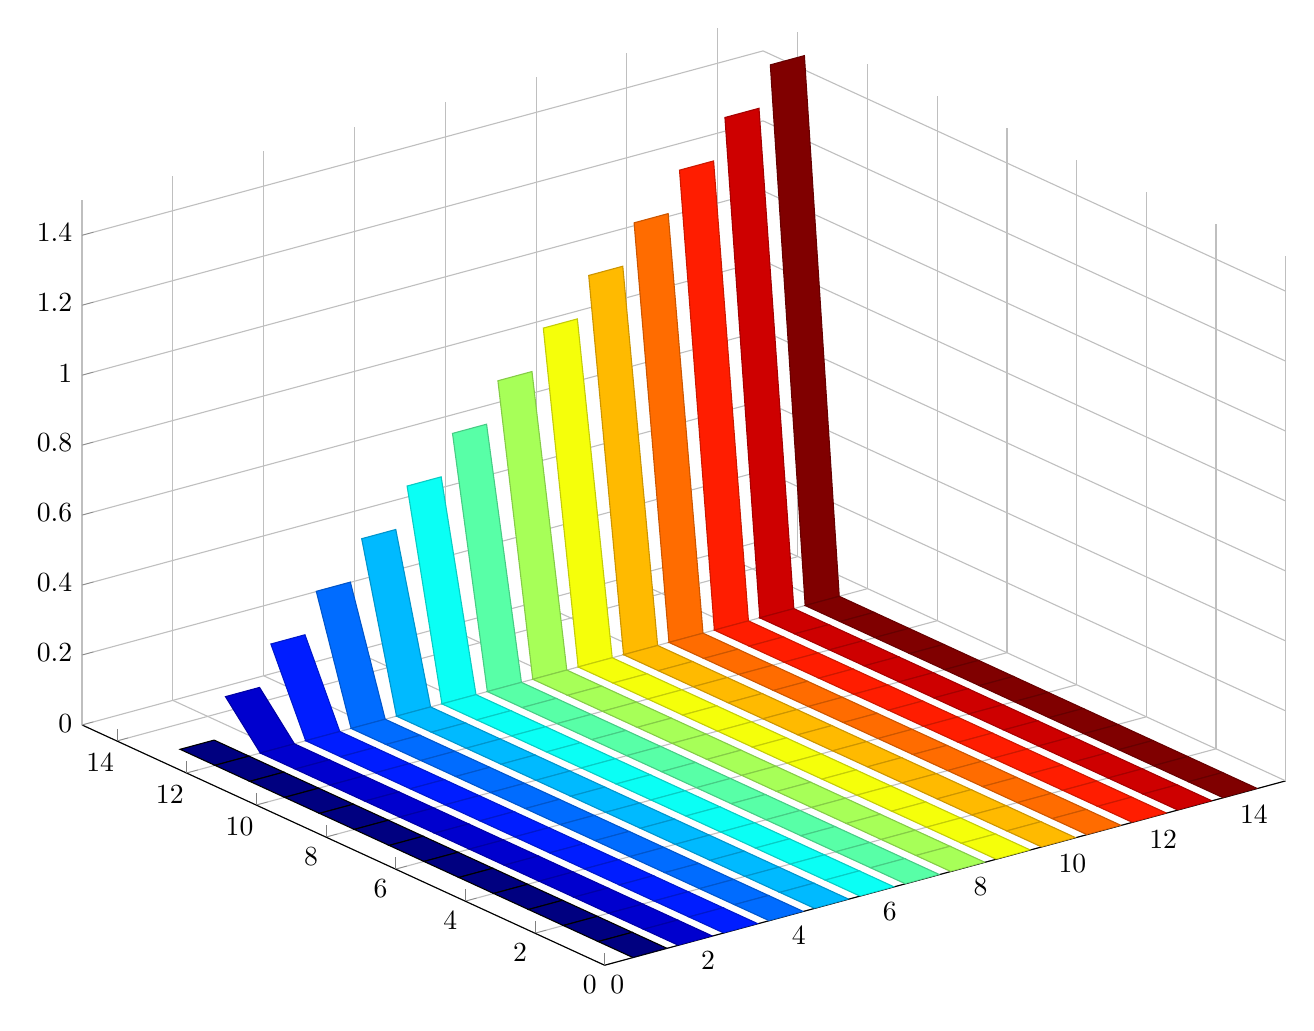
\begin{tikzpicture}

\begin{axis}[%
width=6.01828521434821in,
height=4.74667979002625in,
view={-37.5}{30},
scale only axis,
xmin=0,
xmax=15,
xmajorgrids,
ymin=0,
ymax=15,
ymajorgrids,
zmin=0,
zmax=1.5,
zmajorgrids,
axis x line*=bottom,
axis y line*=left,
axis z line*=left
]

\addplot3[%
surf,
shader=flat corner,
draw=black,
colormap/jet,
point meta=explicit,
mesh/rows=2]
table[row sep=crcr,header=false,meta index=3] {0.625	0	0	1\\
0.625	1	0	1\\
0.625	2	0	1\\
0.625	3	0	1\\
0.625	4	0	1\\
0.625	5	0	1\\
0.625	6	0	1\\
0.625	7	0	1\\
0.625	8	0	1\\
0.625	9	0	1\\
0.625	10	0	1\\
0.625	11	0	1\\
0.625	12	0	1\\
0.625	13	0	1\\
1.375	0	0	1\\
1.375	1	0	1\\
1.375	2	0	1\\
1.375	3	0	1\\
1.375	4	0	1\\
1.375	5	0	1\\
1.375	6	0	1\\
1.375	7	0	1\\
1.375	8	0	1\\
1.375	9	0	1\\
1.375	10	0	1\\
1.375	11	0	1\\
1.375	12	0	1\\
1.375	13	0	1\\
};

\addplot3[%
surf,
shader=faceted,
draw=black,
colormap/jet,
point meta=explicit,
mesh/rows=2]
table[row sep=crcr,header=false,meta index=3] {1.625	0	0	2\\
1.625	1	0	2\\
1.625	2	0	2\\
1.625	3	0	2\\
1.625	4	0	2\\
1.625	5	0	2\\
1.625	6	0	2\\
1.625	7	0	2\\
1.625	8	0	2\\
1.625	9	0	2\\
1.625	10	0	2\\
1.625	11	0	2\\
1.625	12	0	2\\
1.625	13	0.115384615384615	2\\
2.375	0	0	2\\
2.375	1	0	2\\
2.375	2	0	2\\
2.375	3	0	2\\
2.375	4	0	2\\
2.375	5	0	2\\
2.375	6	0	2\\
2.375	7	0	2\\
2.375	8	0	2\\
2.375	9	0	2\\
2.375	10	0	2\\
2.375	11	0	2\\
2.375	12	0	2\\
2.375	13	0.115384615384615	2\\
};

\addplot3[%
surf,
shader=faceted,
draw=black,
colormap/jet,
point meta=explicit,
mesh/rows=2]
table[row sep=crcr,header=false,meta index=3] {2.625	0	0	3\\
2.625	1	0	3\\
2.625	2	0	3\\
2.625	3	0	3\\
2.625	4	0	3\\
2.625	5	0	3\\
2.625	6	0	3\\
2.625	7	0	3\\
2.625	8	0	3\\
2.625	9	0	3\\
2.625	10	0	3\\
2.625	11	0	3\\
2.625	12	0	3\\
2.625	13	0.230769230769231	3\\
3.375	0	0	3\\
3.375	1	0	3\\
3.375	2	0	3\\
3.375	3	0	3\\
3.375	4	0	3\\
3.375	5	0	3\\
3.375	6	0	3\\
3.375	7	0	3\\
3.375	8	0	3\\
3.375	9	0	3\\
3.375	10	0	3\\
3.375	11	0	3\\
3.375	12	0	3\\
3.375	13	0.230769230769231	3\\
};

\addplot3[%
surf,
shader=faceted,
draw=black,
colormap/jet,
point meta=explicit,
mesh/rows=2]
table[row sep=crcr,header=false,meta index=3] {3.625	0	0	4\\
3.625	1	0	4\\
3.625	2	0	4\\
3.625	3	0	4\\
3.625	4	0	4\\
3.625	5	0	4\\
3.625	6	0	4\\
3.625	7	0	4\\
3.625	8	0	4\\
3.625	9	0	4\\
3.625	10	0	4\\
3.625	11	0	4\\
3.625	12	0	4\\
3.625	13	0.346153846153846	4\\
4.375	0	0	4\\
4.375	1	0	4\\
4.375	2	0	4\\
4.375	3	0	4\\
4.375	4	0	4\\
4.375	5	0	4\\
4.375	6	0	4\\
4.375	7	0	4\\
4.375	8	0	4\\
4.375	9	0	4\\
4.375	10	0	4\\
4.375	11	0	4\\
4.375	12	0	4\\
4.375	13	0.346153846153846	4\\
};

\addplot3[%
surf,
shader=faceted,
draw=black,
colormap/jet,
point meta=explicit,
mesh/rows=2]
table[row sep=crcr,header=false,meta index=3] {4.625	0	0	5\\
4.625	1	0	5\\
4.625	2	0	5\\
4.625	3	0	5\\
4.625	4	0	5\\
4.625	5	0	5\\
4.625	6	0	5\\
4.625	7	0	5\\
4.625	8	0	5\\
4.625	9	0	5\\
4.625	10	0	5\\
4.625	11	0	5\\
4.625	12	0	5\\
4.625	13	0.461538461538462	5\\
5.375	0	0	5\\
5.375	1	0	5\\
5.375	2	0	5\\
5.375	3	0	5\\
5.375	4	0	5\\
5.375	5	0	5\\
5.375	6	0	5\\
5.375	7	0	5\\
5.375	8	0	5\\
5.375	9	0	5\\
5.375	10	0	5\\
5.375	11	0	5\\
5.375	12	0	5\\
5.375	13	0.461538461538462	5\\
};

\addplot3[%
surf,
shader=faceted,
draw=black,
colormap/jet,
point meta=explicit,
mesh/rows=2]
table[row sep=crcr,header=false,meta index=3] {5.625	0	0	6\\
5.625	1	0	6\\
5.625	2	0	6\\
5.625	3	0	6\\
5.625	4	0	6\\
5.625	5	0	6\\
5.625	6	0	6\\
5.625	7	0	6\\
5.625	8	0	6\\
5.625	9	0	6\\
5.625	10	0	6\\
5.625	11	0	6\\
5.625	12	0	6\\
5.625	13	0.576923076923077	6\\
6.375	0	0	6\\
6.375	1	0	6\\
6.375	2	0	6\\
6.375	3	0	6\\
6.375	4	0	6\\
6.375	5	0	6\\
6.375	6	0	6\\
6.375	7	0	6\\
6.375	8	0	6\\
6.375	9	0	6\\
6.375	10	0	6\\
6.375	11	0	6\\
6.375	12	0	6\\
6.375	13	0.576923076923077	6\\
};

\addplot3[%
surf,
shader=faceted,
draw=black,
colormap/jet,
point meta=explicit,
mesh/rows=2]
table[row sep=crcr,header=false,meta index=3] {6.625	0	0	7\\
6.625	1	0	7\\
6.625	2	0	7\\
6.625	3	0	7\\
6.625	4	0	7\\
6.625	5	0	7\\
6.625	6	0	7\\
6.625	7	0	7\\
6.625	8	0	7\\
6.625	9	0	7\\
6.625	10	0	7\\
6.625	11	0	7\\
6.625	12	0	7\\
6.625	13	0.692307692307692	7\\
7.375	0	0	7\\
7.375	1	0	7\\
7.375	2	0	7\\
7.375	3	0	7\\
7.375	4	0	7\\
7.375	5	0	7\\
7.375	6	0	7\\
7.375	7	0	7\\
7.375	8	0	7\\
7.375	9	0	7\\
7.375	10	0	7\\
7.375	11	0	7\\
7.375	12	0	7\\
7.375	13	0.692307692307692	7\\
};

\addplot3[%
surf,
shader=faceted,
draw=black,
colormap/jet,
point meta=explicit,
mesh/rows=2]
table[row sep=crcr,header=false,meta index=3] {7.625	0	0	8\\
7.625	1	0	8\\
7.625	2	0	8\\
7.625	3	0	8\\
7.625	4	0	8\\
7.625	5	0	8\\
7.625	6	0	8\\
7.625	7	0	8\\
7.625	8	0	8\\
7.625	9	0	8\\
7.625	10	0	8\\
7.625	11	0	8\\
7.625	12	0	8\\
7.625	13	0.807692307692308	8\\
8.375	0	0	8\\
8.375	1	0	8\\
8.375	2	0	8\\
8.375	3	0	8\\
8.375	4	0	8\\
8.375	5	0	8\\
8.375	6	0	8\\
8.375	7	0	8\\
8.375	8	0	8\\
8.375	9	0	8\\
8.375	10	0	8\\
8.375	11	0	8\\
8.375	12	0	8\\
8.375	13	0.807692307692308	8\\
};

\addplot3[%
surf,
shader=faceted,
draw=black,
colormap/jet,
point meta=explicit,
mesh/rows=2]
table[row sep=crcr,header=false,meta index=3] {8.625	0	0	9\\
8.625	1	0	9\\
8.625	2	0	9\\
8.625	3	0	9\\
8.625	4	0	9\\
8.625	5	0	9\\
8.625	6	0	9\\
8.625	7	0	9\\
8.625	8	0	9\\
8.625	9	0	9\\
8.625	10	0	9\\
8.625	11	0	9\\
8.625	12	0	9\\
8.625	13	0.923076923076923	9\\
9.375	0	0	9\\
9.375	1	0	9\\
9.375	2	0	9\\
9.375	3	0	9\\
9.375	4	0	9\\
9.375	5	0	9\\
9.375	6	0	9\\
9.375	7	0	9\\
9.375	8	0	9\\
9.375	9	0	9\\
9.375	10	0	9\\
9.375	11	0	9\\
9.375	12	0	9\\
9.375	13	0.923076923076923	9\\
};

\addplot3[%
surf,
shader=faceted,
draw=black,
colormap/jet,
point meta=explicit,
mesh/rows=2]
table[row sep=crcr,header=false,meta index=3] {9.625	0	0	10\\
9.625	1	0	10\\
9.625	2	0	10\\
9.625	3	0	10\\
9.625	4	0	10\\
9.625	5	0	10\\
9.625	6	0	10\\
9.625	7	0	10\\
9.625	8	0	10\\
9.625	9	0	10\\
9.625	10	0	10\\
9.625	11	0	10\\
9.625	12	0	10\\
9.625	13	1.03846153846154	10\\
10.375	0	0	10\\
10.375	1	0	10\\
10.375	2	0	10\\
10.375	3	0	10\\
10.375	4	0	10\\
10.375	5	0	10\\
10.375	6	0	10\\
10.375	7	0	10\\
10.375	8	0	10\\
10.375	9	0	10\\
10.375	10	0	10\\
10.375	11	0	10\\
10.375	12	0	10\\
10.375	13	1.03846153846154	10\\
};

\addplot3[%
surf,
shader=faceted,
draw=black,
colormap/jet,
point meta=explicit,
mesh/rows=2]
table[row sep=crcr,header=false,meta index=3] {10.625	0	0	11\\
10.625	1	0	11\\
10.625	2	0	11\\
10.625	3	0	11\\
10.625	4	0	11\\
10.625	5	0	11\\
10.625	6	0	11\\
10.625	7	0	11\\
10.625	8	0	11\\
10.625	9	0	11\\
10.625	10	0	11\\
10.625	11	0	11\\
10.625	12	0	11\\
10.625	13	1.15384615384615	11\\
11.375	0	0	11\\
11.375	1	0	11\\
11.375	2	0	11\\
11.375	3	0	11\\
11.375	4	0	11\\
11.375	5	0	11\\
11.375	6	0	11\\
11.375	7	0	11\\
11.375	8	0	11\\
11.375	9	0	11\\
11.375	10	0	11\\
11.375	11	0	11\\
11.375	12	0	11\\
11.375	13	1.15384615384615	11\\
};

\addplot3[%
surf,
shader=faceted,
draw=black,
colormap/jet,
point meta=explicit,
mesh/rows=2]
table[row sep=crcr,header=false,meta index=3] {11.625	0	0	12\\
11.625	1	0	12\\
11.625	2	0	12\\
11.625	3	0	12\\
11.625	4	0	12\\
11.625	5	0	12\\
11.625	6	0	12\\
11.625	7	0	12\\
11.625	8	0	12\\
11.625	9	0	12\\
11.625	10	0	12\\
11.625	11	0	12\\
11.625	12	0	12\\
11.625	13	1.26923076923077	12\\
12.375	0	0	12\\
12.375	1	0	12\\
12.375	2	0	12\\
12.375	3	0	12\\
12.375	4	0	12\\
12.375	5	0	12\\
12.375	6	0	12\\
12.375	7	0	12\\
12.375	8	0	12\\
12.375	9	0	12\\
12.375	10	0	12\\
12.375	11	0	12\\
12.375	12	0	12\\
12.375	13	1.26923076923077	12\\
};

\addplot3[%
surf,
shader=faceted,
draw=black,
colormap/jet,
point meta=explicit,
mesh/rows=2]
table[row sep=crcr,header=false,meta index=3] {12.625	0	0	13\\
12.625	1	0	13\\
12.625	2	0	13\\
12.625	3	0	13\\
12.625	4	0	13\\
12.625	5	0	13\\
12.625	6	0	13\\
12.625	7	0	13\\
12.625	8	0	13\\
12.625	9	0	13\\
12.625	10	0	13\\
12.625	11	0	13\\
12.625	12	0	13\\
12.625	13	1.38461538461538	13\\
13.375	0	0	13\\
13.375	1	0	13\\
13.375	2	0	13\\
13.375	3	0	13\\
13.375	4	0	13\\
13.375	5	0	13\\
13.375	6	0	13\\
13.375	7	0	13\\
13.375	8	0	13\\
13.375	9	0	13\\
13.375	10	0	13\\
13.375	11	0	13\\
13.375	12	0	13\\
13.375	13	1.38461538461538	13\\
};

\addplot3[%
surf,
shader=faceted,
draw=black,
colormap/jet,
point meta=explicit,
mesh/rows=2]
table[row sep=crcr,header=false,meta index=3] {13.625	0	0	14\\
13.625	1	0	14\\
13.625	2	0	14\\
13.625	3	0	14\\
13.625	4	0	14\\
13.625	5	0	14\\
13.625	6	0	14\\
13.625	7	0	14\\
13.625	8	0	14\\
13.625	9	0	14\\
13.625	10	0	14\\
13.625	11	0	14\\
13.625	12	0	14\\
13.625	13	1.5	14\\
14.375	0	0	14\\
14.375	1	0	14\\
14.375	2	0	14\\
14.375	3	0	14\\
14.375	4	0	14\\
14.375	5	0	14\\
14.375	6	0	14\\
14.375	7	0	14\\
14.375	8	0	14\\
14.375	9	0	14\\
14.375	10	0	14\\
14.375	11	0	14\\
14.375	12	0	14\\
14.375	13	1.5	14\\
};
\end{axis}
\end{tikzpicture}%
\caption{Final Configuration after 20 iterations of message passing with scheduling and correction factor of $1/N$,$z$-sheer=1.5.}
\label{Fig:Ribbons14Initial_z=1.5}
\end{figure}

\begin{figure}[h]
\centering
\scalebox{0.45}{% This file was created by matlab2tikz v0.4.7 running on MATLAB 7.14.
% Copyright (c) 2008--2014, Nico Schlömer <nico.schloemer@gmail.com>
% All rights reserved.
% Minimal pgfplots version: 1.3
% 
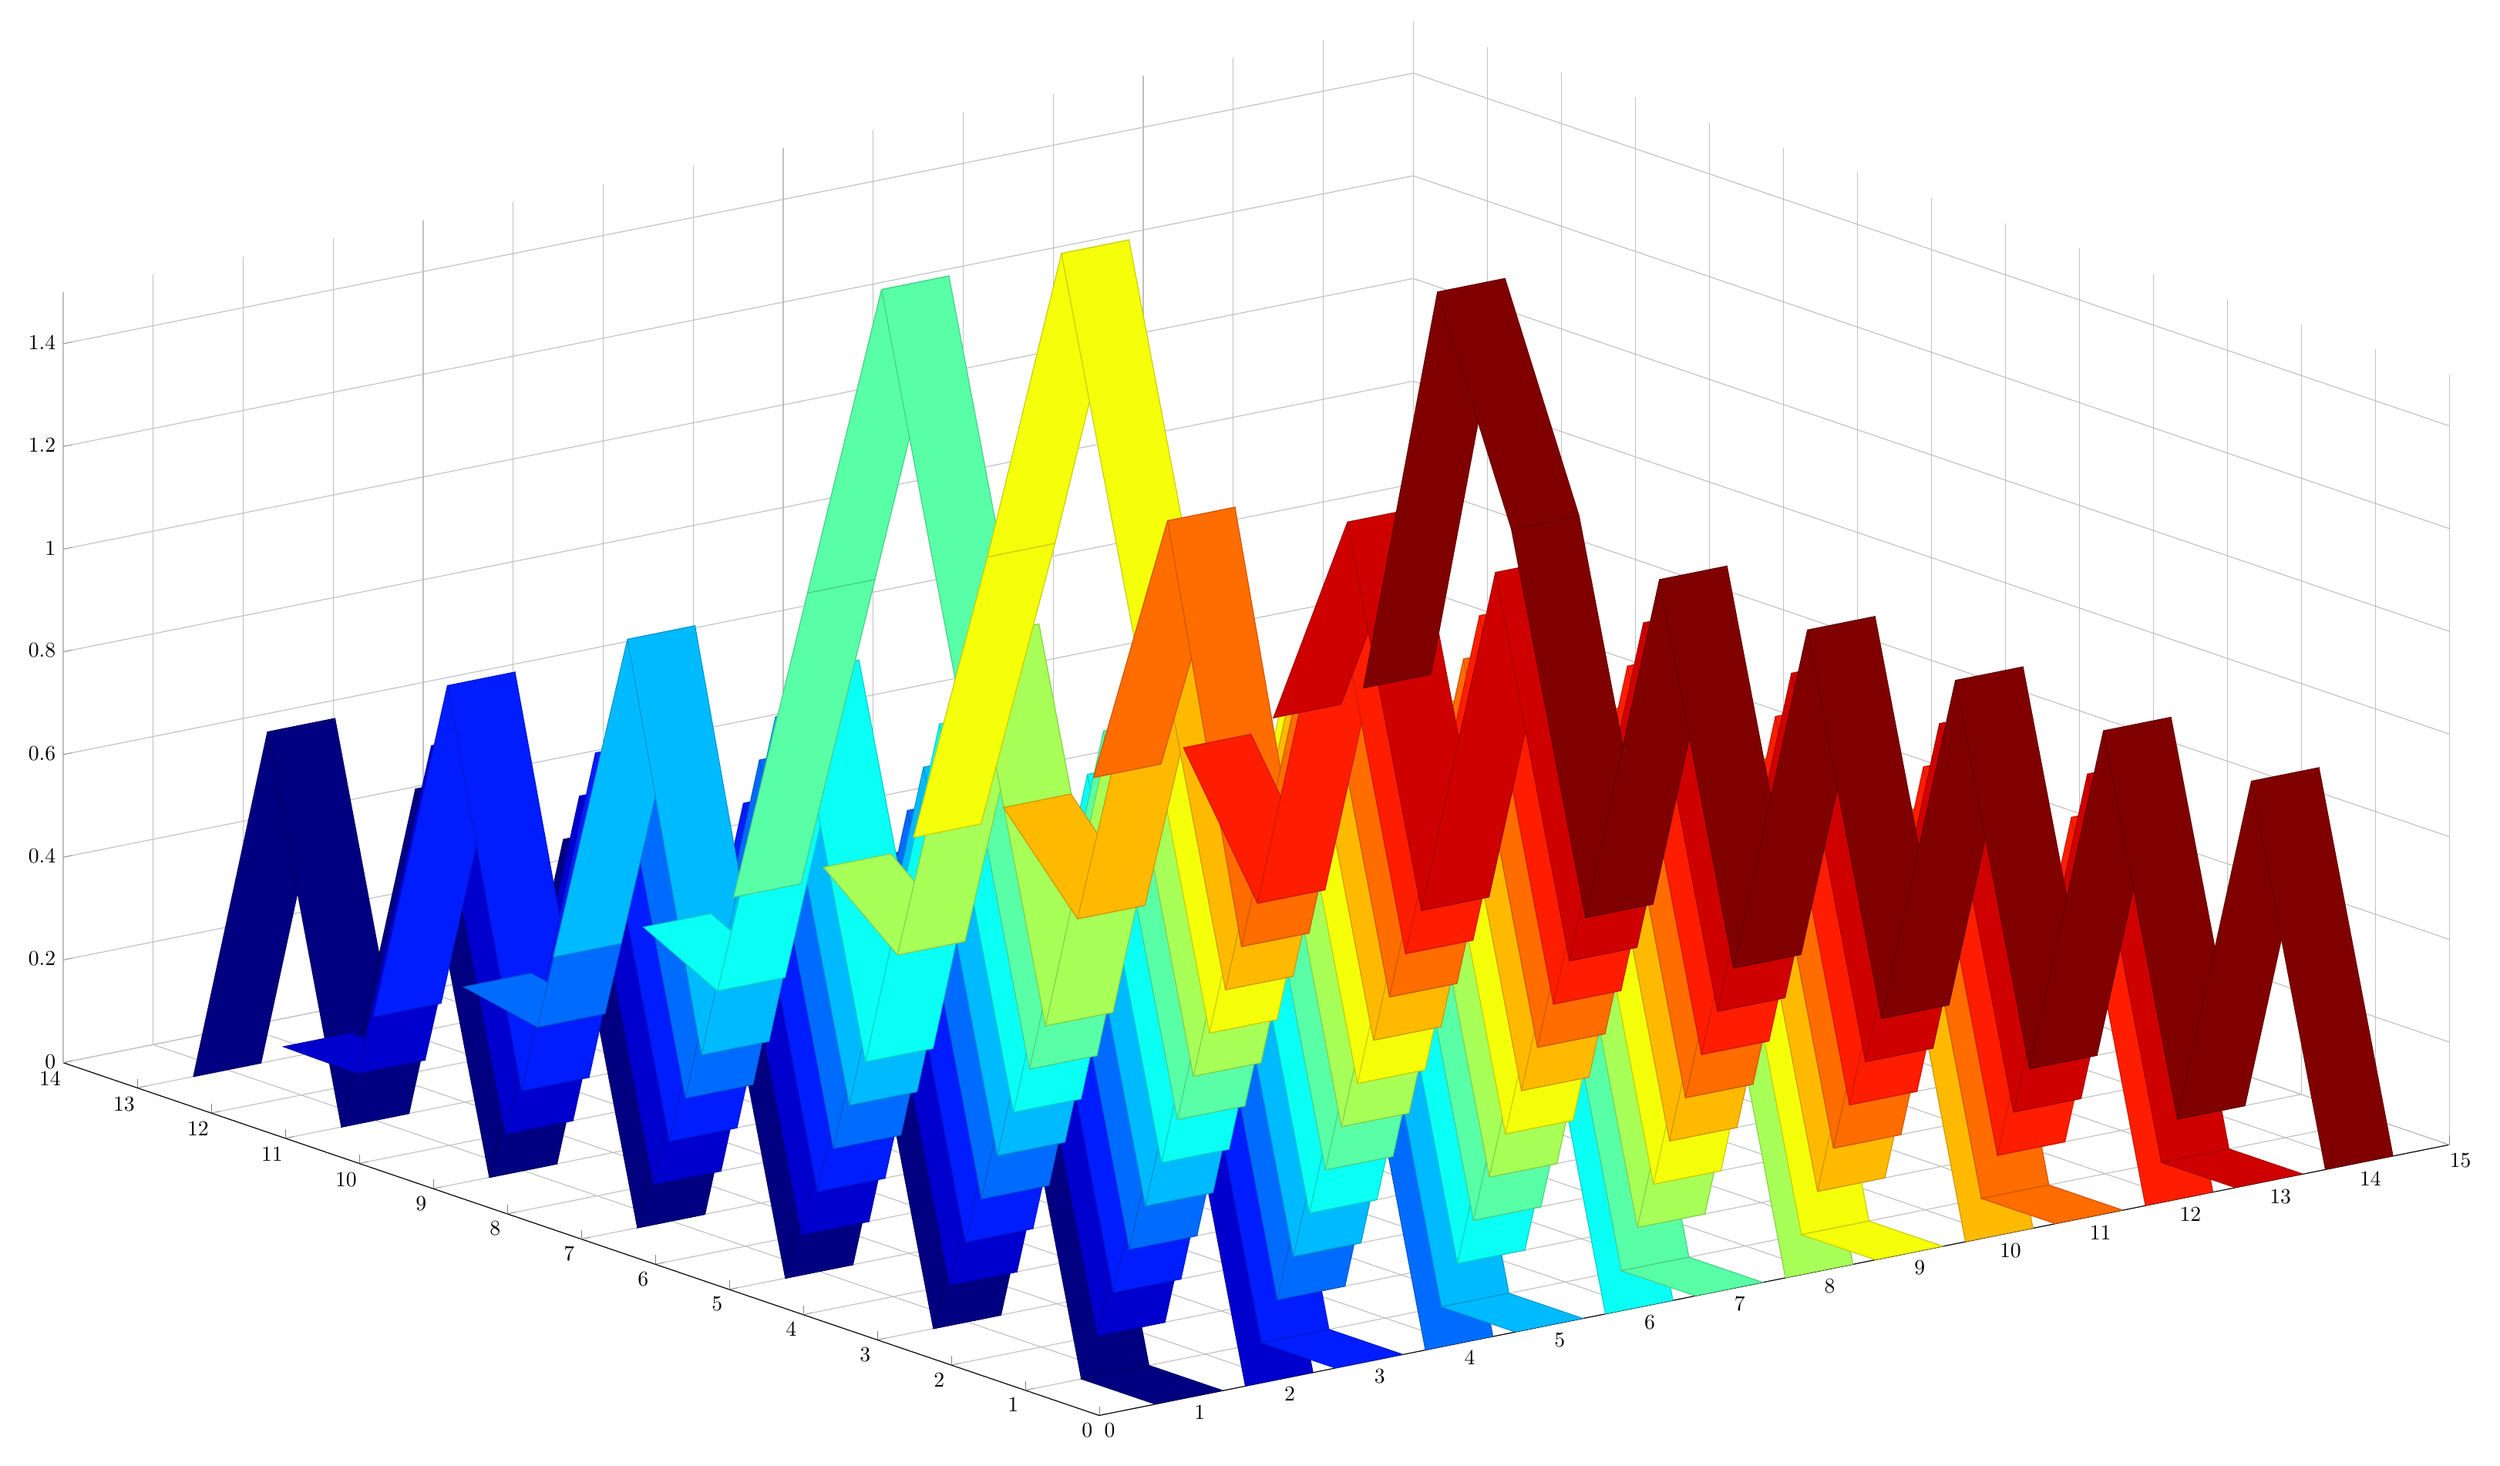
\begin{tikzpicture}

\begin{axis}[%
width=15.4755905511811in,
height=9.04129483814523in,
view={-37.5}{30},
scale only axis,
xmin=0,
xmax=15,
xmajorgrids,
ymin=0,
ymax=14,
ymajorgrids,
zmin=0,
zmax=1.5,
zmajorgrids,
axis x line*=bottom,
axis y line*=left,
axis z line*=left
]

\addplot3[%
surf,
shader=faceted,
draw=black,
colormap/jet,
point meta=explicit,
mesh/rows=2]
table[row sep=crcr,header=false,meta index=3] {0.625	0	0	1\\
0.625	1	0	1\\
0.625	2	0.707106781186547	1\\
0.625	3	0	1\\
0.625	4	0.707106781186547	1\\
0.625	5	0	1\\
0.625	6	0.707106781186547	1\\
0.625	7	0	1\\
0.625	8	0.707106781186547	1\\
0.625	9	0	1\\
0.625	10	0.707106781186547	1\\
0.625	11	0	1\\
0.625	12	0.72	1\\
0.625	13	0	1\\
1.375	0	0	1\\
1.375	1	0	1\\
1.375	2	0.707106781186547	1\\
1.375	3	0	1\\
1.375	4	0.707106781186547	1\\
1.375	5	0	1\\
1.375	6	0.707106781186547	1\\
1.375	7	0	1\\
1.375	8	0.707106781186547	1\\
1.375	9	0	1\\
1.375	10	0.707106781186547	1\\
1.375	11	0	1\\
1.375	12	0.72	1\\
1.375	13	0	1\\
};

\addplot3[%
surf,
shader=faceted,
draw=black,
colormap/jet,
point meta=explicit,
mesh/rows=2]
table[row sep=crcr,header=false,meta index=3] {1.625	0	0	2\\
1.625	1	0.707106781186547	2\\
1.625	2	0	2\\
1.625	3	0.707106781186547	2\\
1.625	4	0	2\\
1.625	5	0.707106781186547	2\\
1.625	6	0	2\\
1.625	7	0.707106781186547	2\\
1.625	8	0	2\\
1.625	9	0.707106781186547	2\\
1.625	10	0	2\\
1.625	11	0.707106781186547	2\\
1.625	12	0.02	2\\
1.625	13	0.0230769230769231	2\\
2.375	0	0	2\\
2.375	1	0.707106781186547	2\\
2.375	2	0	2\\
2.375	3	0.707106781186547	2\\
2.375	4	0	2\\
2.375	5	0.707106781186547	2\\
2.375	6	0	2\\
2.375	7	0.707106781186547	2\\
2.375	8	0	2\\
2.375	9	0.707106781186547	2\\
2.375	10	0	2\\
2.375	11	0.707106781186547	2\\
2.375	12	0.02	2\\
2.375	13	0.0230769230769231	2\\
};

\addplot3[%
surf,
shader=faceted,
draw=black,
colormap/jet,
point meta=explicit,
mesh/rows=2]
table[row sep=crcr,header=false,meta index=3] {2.625	0	0	3\\
2.625	1	0	3\\
2.625	2	0.707106781186547	3\\
2.625	3	0	3\\
2.625	4	0.707106781186547	3\\
2.625	5	0	3\\
2.625	6	0.707106781186547	3\\
2.625	7	0	3\\
2.625	8	0.707106781186547	3\\
2.625	9	0	3\\
2.625	10	0.707106781186547	3\\
2.625	11	0	3\\
2.625	12	0.74	3\\
2.625	13	0.0461538461538461	3\\
3.375	0	0	3\\
3.375	1	0	3\\
3.375	2	0.707106781186547	3\\
3.375	3	0	3\\
3.375	4	0.707106781186547	3\\
3.375	5	0	3\\
3.375	6	0.707106781186547	3\\
3.375	7	0	3\\
3.375	8	0.707106781186547	3\\
3.375	9	0	3\\
3.375	10	0.707106781186547	3\\
3.375	11	0	3\\
3.375	12	0.74	3\\
3.375	13	0.0461538461538461	3\\
};

\addplot3[%
surf,
shader=faceted,
draw=black,
colormap/jet,
point meta=explicit,
mesh/rows=2]
table[row sep=crcr,header=false,meta index=3] {3.625	0	0	4\\
3.625	1	0.707106781186547	4\\
3.625	2	0	4\\
3.625	3	0.707106781186547	4\\
3.625	4	0	4\\
3.625	5	0.707106781186547	4\\
3.625	6	0	4\\
3.625	7	0.707106781186547	4\\
3.625	8	0	4\\
3.625	9	0.707106781186547	4\\
3.625	10	0	4\\
3.625	11	0.707106781186547	4\\
3.625	12	0.04	4\\
3.625	13	0.0692307692307692	4\\
4.375	0	0	4\\
4.375	1	0.707106781186547	4\\
4.375	2	0	4\\
4.375	3	0.707106781186547	4\\
4.375	4	0	4\\
4.375	5	0.707106781186547	4\\
4.375	6	0	4\\
4.375	7	0.707106781186547	4\\
4.375	8	0	4\\
4.375	9	0.707106781186547	4\\
4.375	10	0	4\\
4.375	11	0.707106781186547	4\\
4.375	12	0.04	4\\
4.375	13	0.0692307692307692	4\\
};

\addplot3[%
surf,
shader=faceted,
draw=black,
colormap/jet,
point meta=explicit,
mesh/rows=2]
table[row sep=crcr,header=false,meta index=3] {4.625	0	0	5\\
4.625	1	0	5\\
4.625	2	0.707106781186547	5\\
4.625	3	0	5\\
4.625	4	0.707106781186547	5\\
4.625	5	0	5\\
4.625	6	0.707106781186547	5\\
4.625	7	0	5\\
4.625	8	0.707106781186547	5\\
4.625	9	0	5\\
4.625	10	0.707106781186547	5\\
4.625	11	0	5\\
4.625	12	0.76	5\\
4.625	13	0.0923076923076923	5\\
5.375	0	0	5\\
5.375	1	0	5\\
5.375	2	0.707106781186547	5\\
5.375	3	0	5\\
5.375	4	0.707106781186547	5\\
5.375	5	0	5\\
5.375	6	0.707106781186547	5\\
5.375	7	0	5\\
5.375	8	0.707106781186547	5\\
5.375	9	0	5\\
5.375	10	0.707106781186547	5\\
5.375	11	0	5\\
5.375	12	0.76	5\\
5.375	13	0.0923076923076923	5\\
};

\addplot3[%
surf,
shader=faceted,
draw=black,
colormap/jet,
point meta=explicit,
mesh/rows=2]
table[row sep=crcr,header=false,meta index=3] {5.625	0	0	6\\
5.625	1	0.707106781186547	6\\
5.625	2	0	6\\
5.625	3	0.707106781186547	6\\
5.625	4	0	6\\
5.625	5	0.707106781186547	6\\
5.625	6	0	6\\
5.625	7	0.707106781186547	6\\
5.625	8	0	6\\
5.625	9	0.707106781186547	6\\
5.625	10	0	6\\
5.625	11	0.707106781186547	6\\
5.625	12	0.04	6\\
5.625	13	0.115384615384615	6\\
6.375	0	0	6\\
6.375	1	0.707106781186547	6\\
6.375	2	0	6\\
6.375	3	0.707106781186547	6\\
6.375	4	0	6\\
6.375	5	0.707106781186547	6\\
6.375	6	0	6\\
6.375	7	0.707106781186547	6\\
6.375	8	0	6\\
6.375	9	0.707106781186547	6\\
6.375	10	0	6\\
6.375	11	0.707106781186547	6\\
6.375	12	0.04	6\\
6.375	13	0.115384615384615	6\\
};

\addplot3[%
surf,
shader=faceted,
draw=black,
colormap/jet,
point meta=explicit,
mesh/rows=2]
table[row sep=crcr,header=false,meta index=3] {6.625	0	0	7\\
6.625	1	0	7\\
6.625	2	0.707106781186547	7\\
6.625	3	0	7\\
6.625	4	0.707106781186547	7\\
6.625	5	0	7\\
6.625	6	0.707106781186547	7\\
6.625	7	0	7\\
6.625	8	0.707106781186547	7\\
6.625	9	0	7\\
6.625	10	0.707106781186547	7\\
6.625	11	1.42	7\\
6.625	12	0.78	7\\
6.625	13	0.138461538461538	7\\
7.375	0	0	7\\
7.375	1	0	7\\
7.375	2	0.707106781186547	7\\
7.375	3	0	7\\
7.375	4	0.707106781186547	7\\
7.375	5	0	7\\
7.375	6	0.707106781186547	7\\
7.375	7	0	7\\
7.375	8	0.707106781186547	7\\
7.375	9	0	7\\
7.375	10	0.707106781186547	7\\
7.375	11	1.42	7\\
7.375	12	0.78	7\\
7.375	13	0.138461538461538	7\\
};

\addplot3[%
surf,
shader=faceted,
draw=black,
colormap/jet,
point meta=explicit,
mesh/rows=2]
table[row sep=crcr,header=false,meta index=3] {7.625	0	0	8\\
7.625	1	0.707106781186547	8\\
7.625	2	0	8\\
7.625	3	0.707106781186547	8\\
7.625	4	0	8\\
7.625	5	0.707106781186547	8\\
7.625	6	0	8\\
7.625	7	0.707106781186547	8\\
7.625	8	0	8\\
7.625	9	0.707106781186547	8\\
7.625	10	0	8\\
7.625	11	0.707106781186547	8\\
7.625	12	0.04	8\\
7.625	13	0.161538461538462	8\\
8.375	0	0	8\\
8.375	1	0.707106781186547	8\\
8.375	2	0	8\\
8.375	3	0.707106781186547	8\\
8.375	4	0	8\\
8.375	5	0.707106781186547	8\\
8.375	6	0	8\\
8.375	7	0.707106781186547	8\\
8.375	8	0	8\\
8.375	9	0.707106781186547	8\\
8.375	10	0	8\\
8.375	11	0.707106781186547	8\\
8.375	12	0.04	8\\
8.375	13	0.161538461538462	8\\
};

\addplot3[%
surf,
shader=faceted,
draw=black,
colormap/jet,
point meta=explicit,
mesh/rows=2]
table[row sep=crcr,header=false,meta index=3] {8.625	0	0	9\\
8.625	1	0	9\\
8.625	2	0.707106781186547	9\\
8.625	3	0	9\\
8.625	4	0.707106781186547	9\\
8.625	5	0	9\\
8.625	6	0.707106781186547	9\\
8.625	7	0	9\\
8.625	8	0.707106781186547	9\\
8.625	9	0	9\\
8.625	10	0.707106781186547	9\\
8.625	11	1.42	9\\
8.625	12	0.78	9\\
8.625	13	0.184615384615385	9\\
9.375	0	0	9\\
9.375	1	0	9\\
9.375	2	0.707106781186547	9\\
9.375	3	0	9\\
9.375	4	0.707106781186547	9\\
9.375	5	0	9\\
9.375	6	0.707106781186547	9\\
9.375	7	0	9\\
9.375	8	0.707106781186547	9\\
9.375	9	0	9\\
9.375	10	0.707106781186547	9\\
9.375	11	1.42	9\\
9.375	12	0.78	9\\
9.375	13	0.184615384615385	9\\
};

\addplot3[%
surf,
shader=faceted,
draw=black,
colormap/jet,
point meta=explicit,
mesh/rows=2]
table[row sep=crcr,header=false,meta index=3] {9.625	0	0	10\\
9.625	1	0.707106781186547	10\\
9.625	2	0	10\\
9.625	3	0.707106781186547	10\\
9.625	4	0	10\\
9.625	5	0.707106781186547	10\\
9.625	6	0	10\\
9.625	7	0.707106781186547	10\\
9.625	8	0	10\\
9.625	9	0.707106781186547	10\\
9.625	10	0	10\\
9.625	11	0.707106781186547	10\\
9.625	12	0.04	10\\
9.625	13	0.207692307692308	10\\
10.375	0	0	10\\
10.375	1	0.707106781186547	10\\
10.375	2	0	10\\
10.375	3	0.707106781186547	10\\
10.375	4	0	10\\
10.375	5	0.707106781186547	10\\
10.375	6	0	10\\
10.375	7	0.707106781186547	10\\
10.375	8	0	10\\
10.375	9	0.707106781186547	10\\
10.375	10	0	10\\
10.375	11	0.707106781186547	10\\
10.375	12	0.04	10\\
10.375	13	0.207692307692308	10\\
};

\addplot3[%
surf,
shader=faceted,
draw=black,
colormap/jet,
point meta=explicit,
mesh/rows=2]
table[row sep=crcr,header=false,meta index=3] {10.625	0	0	11\\
10.625	1	0	11\\
10.625	2	0.707106781186547	11\\
10.625	3	0	11\\
10.625	4	0.707106781186547	11\\
10.625	5	0	11\\
10.625	6	0.707106781186547	11\\
10.625	7	0	11\\
10.625	8	0.707106781186547	11\\
10.625	9	0	11\\
10.625	10	0.707106781186547	11\\
10.625	11	0	11\\
10.625	12	0.78	11\\
10.625	13	0.230769230769231	11\\
11.375	0	0	11\\
11.375	1	0	11\\
11.375	2	0.707106781186547	11\\
11.375	3	0	11\\
11.375	4	0.707106781186547	11\\
11.375	5	0	11\\
11.375	6	0.707106781186547	11\\
11.375	7	0	11\\
11.375	8	0.707106781186547	11\\
11.375	9	0	11\\
11.375	10	0.707106781186547	11\\
11.375	11	0	11\\
11.375	12	0.78	11\\
11.375	13	0.230769230769231	11\\
};

\addplot3[%
surf,
shader=faceted,
draw=black,
colormap/jet,
point meta=explicit,
mesh/rows=2]
table[row sep=crcr,header=false,meta index=3] {11.625	0	0	12\\
11.625	1	0.707106781186547	12\\
11.625	2	0	12\\
11.625	3	0.707106781186547	12\\
11.625	4	0	12\\
11.625	5	0.707106781186547	12\\
11.625	6	0	12\\
11.625	7	0.707106781186547	12\\
11.625	8	0	12\\
11.625	9	0.707106781186547	12\\
11.625	10	0	12\\
11.625	11	0.707106781186547	12\\
11.625	12	0	12\\
11.625	13	0.253846153846154	12\\
12.375	0	0	12\\
12.375	1	0.707106781186547	12\\
12.375	2	0	12\\
12.375	3	0.707106781186547	12\\
12.375	4	0	12\\
12.375	5	0.707106781186547	12\\
12.375	6	0	12\\
12.375	7	0.707106781186547	12\\
12.375	8	0	12\\
12.375	9	0.707106781186547	12\\
12.375	10	0	12\\
12.375	11	0.707106781186547	12\\
12.375	12	0	12\\
12.375	13	0.253846153846154	12\\
};

\addplot3[%
surf,
shader=faceted,
draw=black,
colormap/jet,
point meta=explicit,
mesh/rows=2]
table[row sep=crcr,header=false,meta index=3] {12.625	0	0	13\\
12.625	1	0	13\\
12.625	2	0.707106781186547	13\\
12.625	3	0	13\\
12.625	4	0.707106781186547	13\\
12.625	5	0	13\\
12.625	6	0.707106781186547	13\\
12.625	7	0	13\\
12.625	8	0.707106781186547	13\\
12.625	9	0	13\\
12.625	10	0.707106781186547	13\\
12.625	11	0	13\\
12.625	12	0.707106781186547	13\\
12.625	13	0.276923076923077	13\\
13.375	0	0	13\\
13.375	1	0	13\\
13.375	2	0.707106781186547	13\\
13.375	3	0	13\\
13.375	4	0.707106781186547	13\\
13.375	5	0	13\\
13.375	6	0.707106781186547	13\\
13.375	7	0	13\\
13.375	8	0.707106781186547	13\\
13.375	9	0	13\\
13.375	10	0.707106781186547	13\\
13.375	11	0	13\\
13.375	12	0.707106781186547	13\\
13.375	13	0.276923076923077	13\\
};

\addplot3[%
surf,
shader=faceted,
draw=black,
colormap/jet,
point meta=explicit,
mesh/rows=2]
table[row sep=crcr,header=false,meta index=3] {13.625	0	0	14\\
13.625	1	0.707106781186547	14\\
13.625	2	0	14\\
13.625	3	0.707106781186547	14\\
13.625	4	0	14\\
13.625	5	0.707106781186547	14\\
13.625	6	0	14\\
13.625	7	0.707106781186547	14\\
13.625	8	0	14\\
13.625	9	0.707106781186547	14\\
13.625	10	0	14\\
13.625	11	0.707106781186547	14\\
13.625	12	1.12	14\\
13.625	13	0.3	14\\
14.375	0	0	14\\
14.375	1	0.707106781186547	14\\
14.375	2	0	14\\
14.375	3	0.707106781186547	14\\
14.375	4	0	14\\
14.375	5	0.707106781186547	14\\
14.375	6	0	14\\
14.375	7	0.707106781186547	14\\
14.375	8	0	14\\
14.375	9	0.707106781186547	14\\
14.375	10	0	14\\
14.375	11	0.707106781186547	14\\
14.375	12	1.12	14\\
14.375	13	0.3	14\\
};
\end{axis}
\end{tikzpicture}%}
\caption{Final Configuration after 20 iterations of message passing with scheduling and correction factor of $1/N$, $z$-sheer=0.3.}
\label{Fig:Ribbons14Final_z=1.5}
\end{figure}

\begin{figure}[h]
\centering
\scalebox{0.5}{% This file was created by matlab2tikz v0.4.7 running on MATLAB 7.14.
% Copyright (c) 2008--2014, Nico Schlömer <nico.schloemer@gmail.com>
% All rights reserved.
% Minimal pgfplots version: 1.3
% 
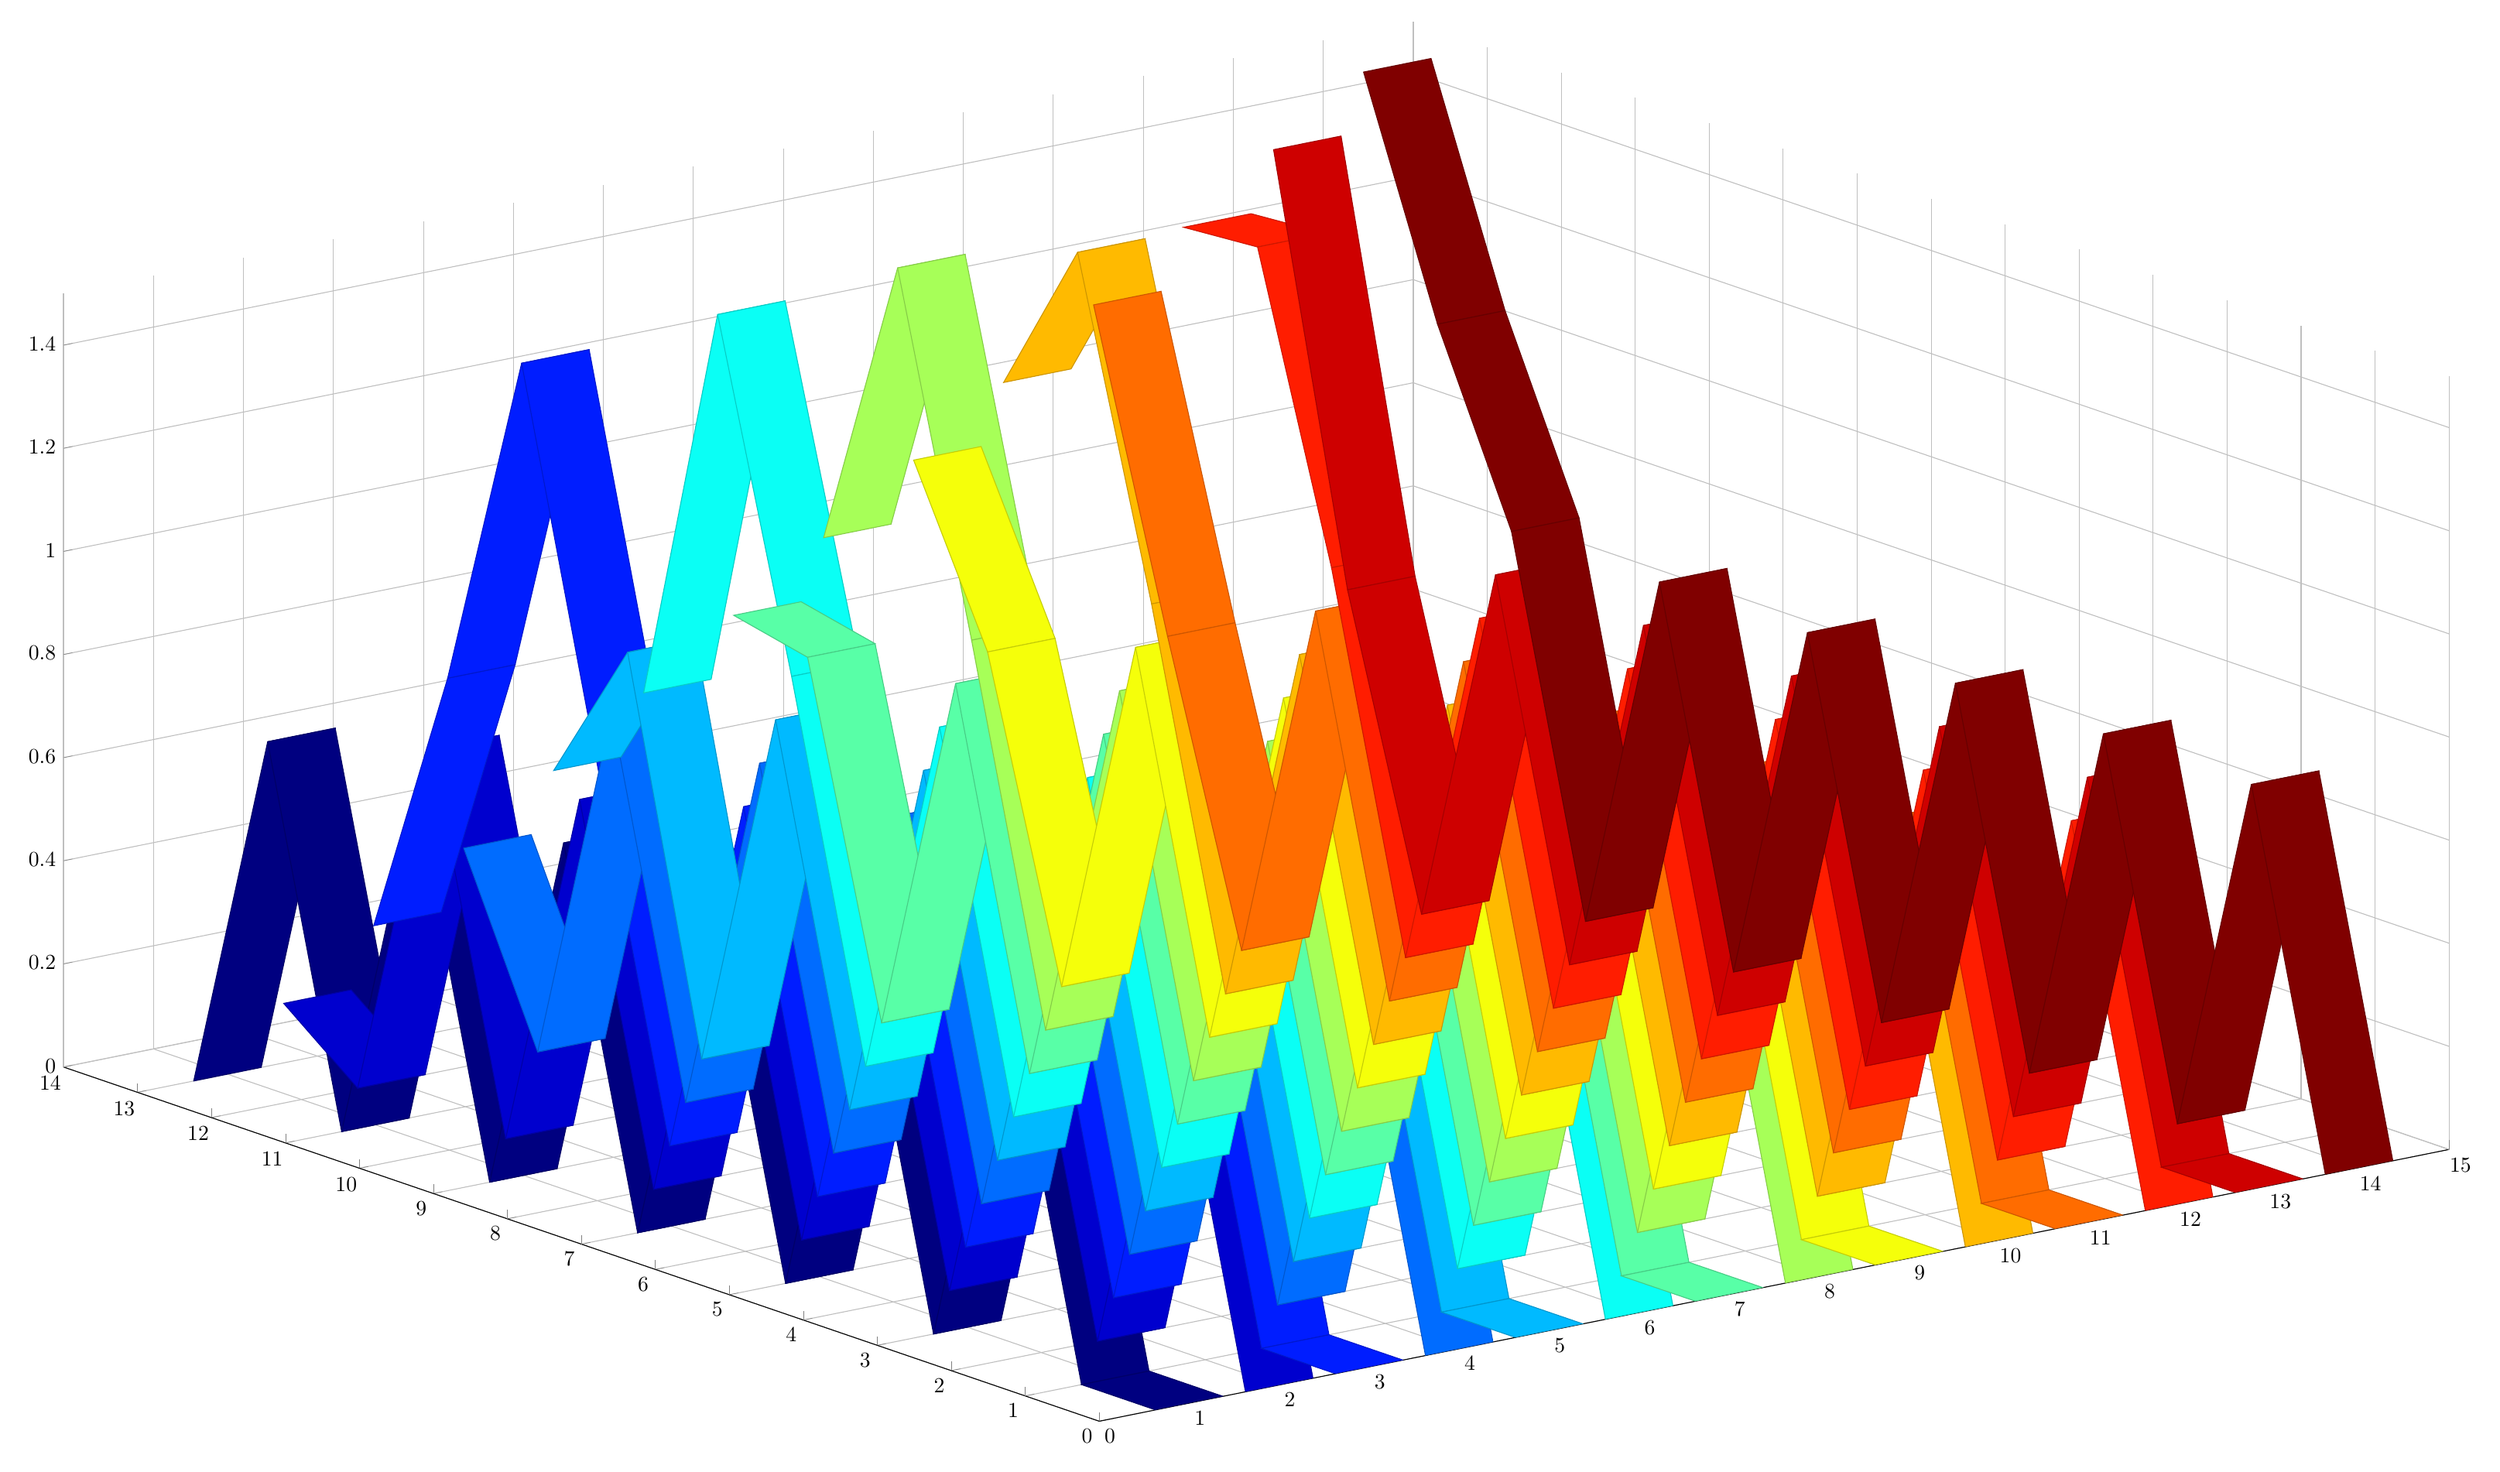
\begin{tikzpicture}

\begin{axis}[%
width=15.4111089238845in,
height=9.04129483814523in,
view={-37.5}{30},
scale only axis,
xmin=0,
xmax=15,
xmajorgrids,
ymin=0,
ymax=14,
ymajorgrids,
zmin=0,
zmax=1.5,
zmajorgrids,
axis x line*=bottom,
axis y line*=left,
axis z line*=left
]

\addplot3[%
surf,
shader=faceted,
draw=black,
colormap/jet,
point meta=explicit,
mesh/rows=2]
table[row sep=crcr,header=false,meta index=3] {0.625	0	0	1\\
0.625	1	0	1\\
0.625	2	0.707106781186547	1\\
0.625	3	0	1\\
0.625	4	0.707106781186547	1\\
0.625	5	0	1\\
0.625	6	0.707106781186547	1\\
0.625	7	0	1\\
0.625	8	0.707106781186547	1\\
0.625	9	0	1\\
0.625	10	0.707106781186547	1\\
0.625	11	0	1\\
0.625	12	0.707106781186547	1\\
0.625	13	0	1\\
1.375	0	0	1\\
1.375	1	0	1\\
1.375	2	0.707106781186547	1\\
1.375	3	0	1\\
1.375	4	0.707106781186547	1\\
1.375	5	0	1\\
1.375	6	0.707106781186547	1\\
1.375	7	0	1\\
1.375	8	0.707106781186547	1\\
1.375	9	0	1\\
1.375	10	0.707106781186547	1\\
1.375	11	0	1\\
1.375	12	0.707106781186547	1\\
1.375	13	0	1\\
};

\addplot3[%
surf,
shader=faceted,
draw=black,
colormap/jet,
point meta=explicit,
mesh/rows=2]
table[row sep=crcr,header=false,meta index=3] {1.625	0	0	2\\
1.625	1	0.707106781186547	2\\
1.625	2	0	2\\
1.625	3	0.707106781186547	2\\
1.625	4	0	2\\
1.625	5	0.707106781186547	2\\
1.625	6	0	2\\
1.625	7	0.707106781186547	2\\
1.625	8	0	2\\
1.625	9	0.707106781186547	2\\
1.625	10	0	2\\
1.625	11	0.707106781186547	2\\
1.625	12	0	2\\
1.625	13	0.115384615384615	2\\
2.375	0	0	2\\
2.375	1	0.707106781186547	2\\
2.375	2	0	2\\
2.375	3	0.707106781186547	2\\
2.375	4	0	2\\
2.375	5	0.707106781186547	2\\
2.375	6	0	2\\
2.375	7	0.707106781186547	2\\
2.375	8	0	2\\
2.375	9	0.707106781186547	2\\
2.375	10	0	2\\
2.375	11	0.707106781186547	2\\
2.375	12	0	2\\
2.375	13	0.115384615384615	2\\
};

\addplot3[%
surf,
shader=faceted,
draw=black,
colormap/jet,
point meta=explicit,
mesh/rows=2]
table[row sep=crcr,header=false,meta index=3] {2.625	0	0	3\\
2.625	1	0	3\\
2.625	2	0.707106781186547	3\\
2.625	3	0	3\\
2.625	4	0.707106781186547	3\\
2.625	5	0	3\\
2.625	6	0.707106781186547	3\\
2.625	7	0	3\\
2.625	8	0.707106781186547	3\\
2.625	9	0	3\\
2.625	10	0.707106781186547	3\\
2.625	11	1.42	3\\
2.625	12	0.76	3\\
2.625	13	0.230769230769231	3\\
3.375	0	0	3\\
3.375	1	0	3\\
3.375	2	0.707106781186547	3\\
3.375	3	0	3\\
3.375	4	0.707106781186547	3\\
3.375	5	0	3\\
3.375	6	0.707106781186547	3\\
3.375	7	0	3\\
3.375	8	0.707106781186547	3\\
3.375	9	0	3\\
3.375	10	0.707106781186547	3\\
3.375	11	1.42	3\\
3.375	12	0.76	3\\
3.375	13	0.230769230769231	3\\
};

\addplot3[%
surf,
shader=faceted,
draw=black,
colormap/jet,
point meta=explicit,
mesh/rows=2]
table[row sep=crcr,header=false,meta index=3] {3.625	0	0	4\\
3.625	1	0.707106781186547	4\\
3.625	2	0	4\\
3.625	3	0.707106781186547	4\\
3.625	4	0	4\\
3.625	5	0.707106781186547	4\\
3.625	6	0	4\\
3.625	7	0.707106781186547	4\\
3.625	8	0	4\\
3.625	9	0.707106781186547	4\\
3.625	10	0	4\\
3.625	11	0.707106781186547	4\\
3.625	12	0	4\\
3.625	13	0.346153846153846	4\\
4.375	0	0	4\\
4.375	1	0.707106781186547	4\\
4.375	2	0	4\\
4.375	3	0.707106781186547	4\\
4.375	4	0	4\\
4.375	5	0.707106781186547	4\\
4.375	6	0	4\\
4.375	7	0.707106781186547	4\\
4.375	8	0	4\\
4.375	9	0.707106781186547	4\\
4.375	10	0	4\\
4.375	11	0.707106781186547	4\\
4.375	12	0	4\\
4.375	13	0.346153846153846	4\\
};

\addplot3[%
surf,
shader=faceted,
draw=black,
colormap/jet,
point meta=explicit,
mesh/rows=2]
table[row sep=crcr,header=false,meta index=3] {4.625	0	0	5\\
4.625	1	0	5\\
4.625	2	0.707106781186547	5\\
4.625	3	0	5\\
4.625	4	0.707106781186547	5\\
4.625	5	0	5\\
4.625	6	0.707106781186547	5\\
4.625	7	0	5\\
4.625	8	0.707106781186547	5\\
4.625	9	0	5\\
4.625	10	0.707106781186547	5\\
4.625	11	0	5\\
4.625	12	0.74	5\\
4.625	13	0.461538461538462	5\\
5.375	0	0	5\\
5.375	1	0	5\\
5.375	2	0.707106781186547	5\\
5.375	3	0	5\\
5.375	4	0.707106781186547	5\\
5.375	5	0	5\\
5.375	6	0.707106781186547	5\\
5.375	7	0	5\\
5.375	8	0.707106781186547	5\\
5.375	9	0	5\\
5.375	10	0.707106781186547	5\\
5.375	11	0	5\\
5.375	12	0.74	5\\
5.375	13	0.461538461538462	5\\
};

\addplot3[%
surf,
shader=faceted,
draw=black,
colormap/jet,
point meta=explicit,
mesh/rows=2]
table[row sep=crcr,header=false,meta index=3] {5.625	0	0	6\\
5.625	1	0.707106781186547	6\\
5.625	2	0	6\\
5.625	3	0.707106781186547	6\\
5.625	4	0	6\\
5.625	5	0.707106781186547	6\\
5.625	6	0	6\\
5.625	7	0.707106781186547	6\\
5.625	8	0	6\\
5.625	9	0.707106781186547	6\\
5.625	10	0	6\\
5.625	11	0.707106781186547	6\\
5.625	12	1.36	6\\
5.625	13	0.576923076923077	6\\
6.375	0	0	6\\
6.375	1	0.707106781186547	6\\
6.375	2	0	6\\
6.375	3	0.707106781186547	6\\
6.375	4	0	6\\
6.375	5	0.707106781186547	6\\
6.375	6	0	6\\
6.375	7	0.707106781186547	6\\
6.375	8	0	6\\
6.375	9	0.707106781186547	6\\
6.375	10	0	6\\
6.375	11	0.707106781186547	6\\
6.375	12	1.36	6\\
6.375	13	0.576923076923077	6\\
};

\addplot3[%
surf,
shader=faceted,
draw=black,
colormap/jet,
point meta=explicit,
mesh/rows=2]
table[row sep=crcr,header=false,meta index=3] {6.625	0	0	7\\
6.625	1	0	7\\
6.625	2	0.707106781186547	7\\
6.625	3	0	7\\
6.625	4	0.707106781186547	7\\
6.625	5	0	7\\
6.625	6	0.707106781186547	7\\
6.625	7	0	7\\
6.625	8	0.707106781186547	7\\
6.625	9	0	7\\
6.625	10	0.707106781186547	7\\
6.625	11	0	7\\
6.625	12	0.66	7\\
6.625	13	0.692307692307692	7\\
7.375	0	0	7\\
7.375	1	0	7\\
7.375	2	0.707106781186547	7\\
7.375	3	0	7\\
7.375	4	0.707106781186547	7\\
7.375	5	0	7\\
7.375	6	0.707106781186547	7\\
7.375	7	0	7\\
7.375	8	0.707106781186547	7\\
7.375	9	0	7\\
7.375	10	0.707106781186547	7\\
7.375	11	0	7\\
7.375	12	0.66	7\\
7.375	13	0.692307692307692	7\\
};

\addplot3[%
surf,
shader=faceted,
draw=black,
colormap/jet,
point meta=explicit,
mesh/rows=2]
table[row sep=crcr,header=false,meta index=3] {7.625	0	0	8\\
7.625	1	0.707106781186547	8\\
7.625	2	0	8\\
7.625	3	0.707106781186547	8\\
7.625	4	0	8\\
7.625	5	0.707106781186547	8\\
7.625	6	0	8\\
7.625	7	0.707106781186547	8\\
7.625	8	0	8\\
7.625	9	0.707106781186547	8\\
7.625	10	0	8\\
7.625	11	0.707106781186547	8\\
7.625	12	1.38	8\\
7.625	13	0.807692307692308	8\\
8.375	0	0	8\\
8.375	1	0.707106781186547	8\\
8.375	2	0	8\\
8.375	3	0.707106781186547	8\\
8.375	4	0	8\\
8.375	5	0.707106781186547	8\\
8.375	6	0	8\\
8.375	7	0.707106781186547	8\\
8.375	8	0	8\\
8.375	9	0.707106781186547	8\\
8.375	10	0	8\\
8.375	11	0.707106781186547	8\\
8.375	12	1.38	8\\
8.375	13	0.807692307692308	8\\
};

\addplot3[%
surf,
shader=faceted,
draw=black,
colormap/jet,
point meta=explicit,
mesh/rows=2]
table[row sep=crcr,header=false,meta index=3] {8.625	0	0	9\\
8.625	1	0	9\\
8.625	2	0.707106781186547	9\\
8.625	3	0	9\\
8.625	4	0.707106781186547	9\\
8.625	5	0	9\\
8.625	6	0.707106781186547	9\\
8.625	7	0	9\\
8.625	8	0.707106781186547	9\\
8.625	9	0	9\\
8.625	10	0.707106781186547	9\\
8.625	11	0	9\\
8.625	12	0.6	9\\
8.625	13	0.923076923076923	9\\
9.375	0	0	9\\
9.375	1	0	9\\
9.375	2	0.707106781186547	9\\
9.375	3	0	9\\
9.375	4	0.707106781186547	9\\
9.375	5	0	9\\
9.375	6	0.707106781186547	9\\
9.375	7	0	9\\
9.375	8	0.707106781186547	9\\
9.375	9	0	9\\
9.375	10	0.707106781186547	9\\
9.375	11	0	9\\
9.375	12	0.6	9\\
9.375	13	0.923076923076923	9\\
};

\addplot3[%
surf,
shader=faceted,
draw=black,
colormap/jet,
point meta=explicit,
mesh/rows=2]
table[row sep=crcr,header=false,meta index=3] {9.625	0	0	10\\
9.625	1	0.707106781186547	10\\
9.625	2	0	10\\
9.625	3	0.707106781186547	10\\
9.625	4	0	10\\
9.625	5	0.707106781186547	10\\
9.625	6	0	10\\
9.625	7	0.707106781186547	10\\
9.625	8	0	10\\
9.625	9	0.707106781186547	10\\
9.625	10	0	10\\
9.625	11	0.707106781186547	10\\
9.625	12	1.34	10\\
9.625	13	1.03846153846154	10\\
10.375	0	0	10\\
10.375	1	0.707106781186547	10\\
10.375	2	0	10\\
10.375	3	0.707106781186547	10\\
10.375	4	0	10\\
10.375	5	0.707106781186547	10\\
10.375	6	0	10\\
10.375	7	0.707106781186547	10\\
10.375	8	0	10\\
10.375	9	0.707106781186547	10\\
10.375	10	0	10\\
10.375	11	0.707106781186547	10\\
10.375	12	1.34	10\\
10.375	13	1.03846153846154	10\\
};

\addplot3[%
surf,
shader=faceted,
draw=black,
colormap/jet,
point meta=explicit,
mesh/rows=2]
table[row sep=crcr,header=false,meta index=3] {10.625	0	0	11\\
10.625	1	0	11\\
10.625	2	0.707106781186547	11\\
10.625	3	0	11\\
10.625	4	0.707106781186547	11\\
10.625	5	0	11\\
10.625	6	0.707106781186547	11\\
10.625	7	0	11\\
10.625	8	0.707106781186547	11\\
10.625	9	0	11\\
10.625	10	0.707106781186547	11\\
10.625	11	0	11\\
10.625	12	0.56	11\\
10.625	13	1.15384615384615	11\\
11.375	0	0	11\\
11.375	1	0	11\\
11.375	2	0.707106781186547	11\\
11.375	3	0	11\\
11.375	4	0.707106781186547	11\\
11.375	5	0	11\\
11.375	6	0.707106781186547	11\\
11.375	7	0	11\\
11.375	8	0.707106781186547	11\\
11.375	9	0	11\\
11.375	10	0.707106781186547	11\\
11.375	11	0	11\\
11.375	12	0.56	11\\
11.375	13	1.15384615384615	11\\
};

\addplot3[%
surf,
shader=faceted,
draw=black,
colormap/jet,
point meta=explicit,
mesh/rows=2]
table[row sep=crcr,header=false,meta index=3] {11.625	0	0	12\\
11.625	1	0.707106781186547	12\\
11.625	2	0	12\\
11.625	3	0.707106781186547	12\\
11.625	4	0	12\\
11.625	5	0.707106781186547	12\\
11.625	6	0	12\\
11.625	7	0.707106781186547	12\\
11.625	8	0	12\\
11.625	9	0.707106781186547	12\\
11.625	10	0	12\\
11.625	11	0.707106781186547	12\\
11.625	12	1.28	12\\
11.625	13	1.26923076923077	12\\
12.375	0	0	12\\
12.375	1	0.707106781186547	12\\
12.375	2	0	12\\
12.375	3	0.707106781186547	12\\
12.375	4	0	12\\
12.375	5	0.707106781186547	12\\
12.375	6	0	12\\
12.375	7	0.707106781186547	12\\
12.375	8	0	12\\
12.375	9	0.707106781186547	12\\
12.375	10	0	12\\
12.375	11	0.707106781186547	12\\
12.375	12	1.28	12\\
12.375	13	1.26923076923077	12\\
};

\addplot3[%
surf,
shader=faceted,
draw=black,
colormap/jet,
point meta=explicit,
mesh/rows=2]
table[row sep=crcr,header=false,meta index=3] {12.625	0	0	13\\
12.625	1	0	13\\
12.625	2	0.707106781186547	13\\
12.625	3	0	13\\
12.625	4	0.707106781186547	13\\
12.625	5	0	13\\
12.625	6	0.707106781186547	13\\
12.625	7	0	13\\
12.625	8	0.707106781186547	13\\
12.625	9	0	13\\
12.625	10	0.707106781186547	13\\
12.625	11	0	13\\
12.625	12	0.58	13\\
12.625	13	1.38461538461538	13\\
13.375	0	0	13\\
13.375	1	0	13\\
13.375	2	0.707106781186547	13\\
13.375	3	0	13\\
13.375	4	0.707106781186547	13\\
13.375	5	0	13\\
13.375	6	0.707106781186547	13\\
13.375	7	0	13\\
13.375	8	0.707106781186547	13\\
13.375	9	0	13\\
13.375	10	0.707106781186547	13\\
13.375	11	0	13\\
13.375	12	0.58	13\\
13.375	13	1.38461538461538	13\\
};

\addplot3[%
surf,
shader=faceted,
draw=black,
colormap/jet,
point meta=explicit,
mesh/rows=2]
table[row sep=crcr,header=false,meta index=3] {13.625	0	0	14\\
13.625	1	0.707106781186547	14\\
13.625	2	0	14\\
13.625	3	0.707106781186547	14\\
13.625	4	0	14\\
13.625	5	0.707106781186547	14\\
13.625	6	0	14\\
13.625	7	0.707106781186547	14\\
13.625	8	0	14\\
13.625	9	0.707106781186547	14\\
13.625	10	0	14\\
13.625	11	0.707106781186547	14\\
13.625	12	1.06	14\\
13.625	13	1.5	14\\
14.375	0	0	14\\
14.375	1	0.707106781186547	14\\
14.375	2	0	14\\
14.375	3	0.707106781186547	14\\
14.375	4	0	14\\
14.375	5	0.707106781186547	14\\
14.375	6	0	14\\
14.375	7	0.707106781186547	14\\
14.375	8	0	14\\
14.375	9	0.707106781186547	14\\
14.375	10	0	14\\
14.375	11	0.707106781186547	14\\
14.375	12	1.06	14\\
14.375	13	1.5	14\\
};
\end{axis}
\end{tikzpicture}%}
\caption{Final Configuration after 20 iterations of message passing with scheduling and correction factor of $1/N$, $z$-sheer=1.5.}
\label{Fig:Ribbons14Final_z=1.5}
\end{figure}


\begin{figure}
\centering
\scalebox{0.75}{% This file was created by matlab2tikz v0.4.7 running on MATLAB 7.14.
% Copyright (c) 2008--2014, Nico Schlömer <nico.schloemer@gmail.com>
% All rights reserved.
% Minimal pgfplots version: 1.3
% 
\begin{tikzpicture}

\begin{axis}[%
width=7.90974628171479in,
height=4.91620406824147in,
scale only axis,
xmin=0,
xmax=20,
xlabel={\large{Number of Iterations}},
ymin=-90,
ymax=0,
ylabel={\large{Energy of the System}},
legend style={at={(0.604990734246013,0.678315204402839)},anchor=south west,draw=black,fill=white,legend cell align=left}
]
\addplot [color=blue,solid]
  table[row sep=crcr]{1	0\\
2	-10.0990596517374\\
3	-16.5964932777622\\
4	-23.6087624980873\\
5	-30.3699097297178\\
6	-37.1199097297178\\
7	-43.8732855851986\\
8	-50.6232855851986\\
9	-57.3732855851986\\
10	-64.1232855851986\\
11	-70.8732855851986\\
12	-77.6232855851986\\
13	-80.8732855851986\\
14	-80.8732855851986\\
15	-80.8732855851986\\
16	-80.8732855851986\\
17	-80.8732855851986\\
18	-80.8732855851986\\
19	-80.8732855851986\\
20	-80.8732855851986\\
21	-80.8732855851986\\
};
\addlegendentry{\large{Z-Sheer=0.3}};

\addplot [color=red,only marks,mark=asterisk,mark options={solid}]
  table[row sep=crcr]{1	0\\
2	-10.384002574521\\
3	-17.0790631714407\\
4	-23.8290631714407\\
5	-30.5807350269215\\
6	-37.3307350269215\\
7	-44.0807350269215\\
8	-50.8307350269215\\
9	-57.5807350269215\\
10	-64.3307350269215\\
11	-71.0807350269215\\
12	-77.8307350269215\\
13	-81.0807350269215\\
14	-81.0807350269215\\
15	-81.0807350269215\\
16	-81.0807350269215\\
17	-81.0807350269215\\
18	-81.0807350269215\\
19	-81.0807350269215\\
20	-81.0807350269215\\
21	-81.0807350269215\\
};
\addlegendentry{\large{Z-Sheer=0.75}};

\addplot [color=black,only marks,mark=+,mark options={solid}]
  table[row sep=crcr]{1	0\\
2	-10.2204287898\\
3	-16.9285499439927\\
4	-21.5554567978048\\
5	-28.3527204241243\\
6	-36.3209176327974\\
7	-42.0507471055541\\
8	-49.8899771978808\\
9	-56.7571442132372\\
10	-63.4252072846865\\
11	-70.4121316737623\\
12	-77.1323305162204\\
13	-80.435679526043\\
14	-80.4472764652782\\
15	-80.4472764652782\\
16	-80.4472764652782\\
17	-80.4472764652782\\
18	-80.4472764652782\\
19	-80.4472764652782\\
20	-80.4472764652782\\
21	-80.4472764652782\\
};
\addlegendentry{\large{Z-Sheer=1.25}};

\addplot [color=green,dash pattern=on 1pt off 3pt on 3pt off 3pt,mark=square,mark options={solid}]
  table[row sep=crcr]{1	0\\
2	-10.4593927245117\\
3	-15.2134682290899\\
4	-21.977132680779\\
5	-28.6332689806509\\
6	-35.4145086964596\\
7	-42.1336962396141\\
8	-48.8836962396141\\
9	-55.6336962396141\\
10	-62.3836962396141\\
11	-69.1336962396141\\
12	-75.8836962396141\\
13	-79.1336962396141\\
14	-79.1336962396141\\
15	-79.1336962396141\\
16	-79.1336962396141\\
17	-79.1336962396141\\
18	-79.1336962396141\\
19	-79.1336962396141\\
20	-79.1336962396141\\
21	-79.1336962396141\\
};
\addlegendentry\large{{Z-Sheer=2.5}};

\end{axis}
\end{tikzpicture}%}
\caption{Total energy output of the algorithm versus the sheer in Z-direction.}
\label{Fig:Effect_Increasing_Force}
\end{figure}

\bibliographystyle{IEEEtran}
\bibliography{References}

\end{document}	
